\documentclass{article}

\usepackage{neurips_2026}

\usepackage[utf8]{inputenc}
\usepackage[T1]{fontenc}
\usepackage{hyperref}
\usepackage{url}
\usepackage{booktabs}
\usepackage{amsfonts}
\usepackage{amsmath}
\usepackage{amssymb}
\usepackage{nicefrac}
\usepackage{microtype}
\usepackage{xcolor}
\usepackage{graphicx}
\usepackage{subcaption}
\usepackage{multirow}
\usepackage{enumitem}
\usepackage{pgfplots}
\pgfplotsset{compat=1.18}
\usepackage{algorithm}
\usepackage{algpseudocode}

\newcommand{\todo}[1]{\textcolor{red}{\textbf{[TODO: #1]}}}
\newcommand{\am}[1]{\textcolor{blue}{{[aneesh: #1]}}}
\newcommand{\dc}[1]{\textcolor{teal}{{[dylan: #1]}}}
\newcommand{\Kset}{\{1,2,3,4\}}
\newcommand{\pigate}{\pi_{\mathrm{gate}}}


\title{Finding the Time to Think: \\ Adaptive MCTS in Real-Time RL}

%Reinforcement learning for budgeting MCTS planning under real-time

%Reinforcement learning for budgeting computation in real-time

\author{\todo{Author list}}


\begin{document}

\maketitle

% =============================================================================
\begin{abstract}
% =============================================================================
%X What are we doing
Deliberating takes time. In real-time settings, that time is not free.
Standard reinforcement learning (RL) sidesteps this as the environment waits indefinitely
for the agent's decision.
Instead, here, we study environments that progress while waiting for the agent's action, which naturally creates a \textit{cost of deliberation}.
%Y why is this hard
Crucially, there are state-dependent trade-offs between deliberating longer and reacting quickly. Furthermore, deliberating how much to deliberate, in the limit, risks complete paralysis.
% Z our genius insight
We resolve this with a two-step process.
First, we train a standard MCTS policy.
Second, we train a \textit{lightweight} gating policy that decides how many search steps to invest at each state. Our gating policy consistently outperforms fixed-budget baselines and hand-coded heuristics while using less average compute.
We validate the full pipeline in a true two-GPU real-time setup across real-time Pac-Man, Tetris, Snake, Speed Hex, and Speed Go.

\end{abstract}


% =============================================================================
\begin{abstract}
% =============================================================================
%X What are we doing
Deliberating takes time. In real-time settings, that time is not free.
Standard reinforcement learning (RL) sidesteps this as the environment waits indefinitely
for the agent's decision.
Instead, here, we study environments that progress while waiting for the agent's action, which naturally creates a \textit{cost of deliberation}.
%Y why is this hard
Crucially, there are state-dependent trade-offs between deliberating longer and reacting quickly. Furthermore, deliberating how much to deliberate, in the limit, risks complete paralysis.
% Z our genius insight
We resolve this with a two-step process.
First, we train a standard MCTS policy.
Second, we train a \textit{lightweight} gating policy that decides how many search steps to invest at each state. Our gating policy consistently outperforms fixed-budget baselines and hand-coded heuristics while using less average compute.
We validate the full pipeline in a true two-GPU real-time setup across real-time Pac-Man, Tetris, Snake, Speed Hex, and Speed Go.

\end{abstract}

\section{Introduction}
% =============================================================================

Real-world decision-makers operate under time pressure.
In speed chess, the world does not pause while a player thinks: the clock
runs, the opponent's plan develops, and a strong move played too late may be
worse than a weaker move played on time.
Standard reinforcement learning (RL) sidesteps this entirely.
The Markov Decision Process (MDP) framework assumes the environment waits for
the agent, so deliberation is free and an agent may take arbitrarily long to
choose an action.

This assumption breaks down in real-time settings, where the world keeps
progressing while the agent decides.
The cost of deliberation in such settings is not abstract compute usage or
latency in isolation, but \emph{environmental progression}: ghosts close in,
pieces fall, clocks deplete.
A perfect action that arrives one frame too late may be worse than a timely,
good-enough action.

This creates a spectrum of regimes.
At one extreme, the agent reacts immediately to every frame.
At the other, it thinks deeply and falls behind while the environment
continues to evolve.
We study the intermediate regime in which the agent dynamically chooses how
long to think before acting.
We refer to this setting as \emph{variable-delay real-time RL}.

We instantiate this regime with planning-based agents.
Specifically, we use AlphaZero-style models~\citep{silver2018general} that run
Monte Carlo Tree Search (MCTS) at decision time to improve action selection
(see Appendix~\ref{app:az_primer} for a complete description).
The number of MCTS simulations is a natural planning-budget knob: more
simulations can improve the action estimate, but they also take longer to run.
We verify empirically that planning quality and inference latency co-scale over
the simulation ranges we study (Figure~\ref{fig:scaling}).
This makes simulation count the central resource-allocation decision in the
real-time setting.

The key problem is therefore \emph{metareasoning}: deciding not only what
action to take, but how much computation that decision deserves.
We address this with a lightweight \emph{gating policy}, trained with PPO on
top of a \emph{frozen} AlphaZero planner, that maps each state to a budget
$K \in \Kset$.
While the planner runs, the agent executes fast filler actions: reflex actions
in committed-action environments and no-ops in clock environments.
The gate's forward pass is orders of magnitude cheaper than MCTS, so the
meta-decision itself adds negligible real-time cost.

We study this setting across two environment classes.
In \emph{committed-action environments} (Pac-Man, real-time Tetris, Snake), the
world evolves while planning is in progress.
In \emph{clock environments} (Speed Hex, Speed Go), the board is static while
thinking, but each player has an explicit clock that depletes with deliberation.
Both settings make the cost of thinking real by construction, though through
different physical mechanisms.

Our contributions are:
\begin{enumerate}
  \item \textbf{Variable-delay real-time RL.}
    We study a setting in which the agent chooses how long to deliberate at
    each decision point, and instantiate it through two environment classes:
    committed-action progression and explicit clocks.
  \item \textbf{Adaptive gating for MCTS budgets.}
    We train a lightweight gating policy on top of a frozen AlphaZero planner
    that selects a state-dependent planning budget $K \in \Kset$.
  \item \textbf{Empirical and deployment validation.}
    Across five environments, the gating policy outperforms fixed-budget and
    heuristic baselines, and the learned policy transfers directly to true
    two-GPU asynchronous deployment with no architectural change.
\end{enumerate}

The learned strategies are interpretable and state-dependent: the gate plans
more deeply in high-stakes situations and reacts quickly elsewhere.
In a true two-GPU deployment, the same trained policy transfers cleanly, and
gate inference adds negligible overhead relative to MCTS latency.

\begin{figure}[t]
  \centering
  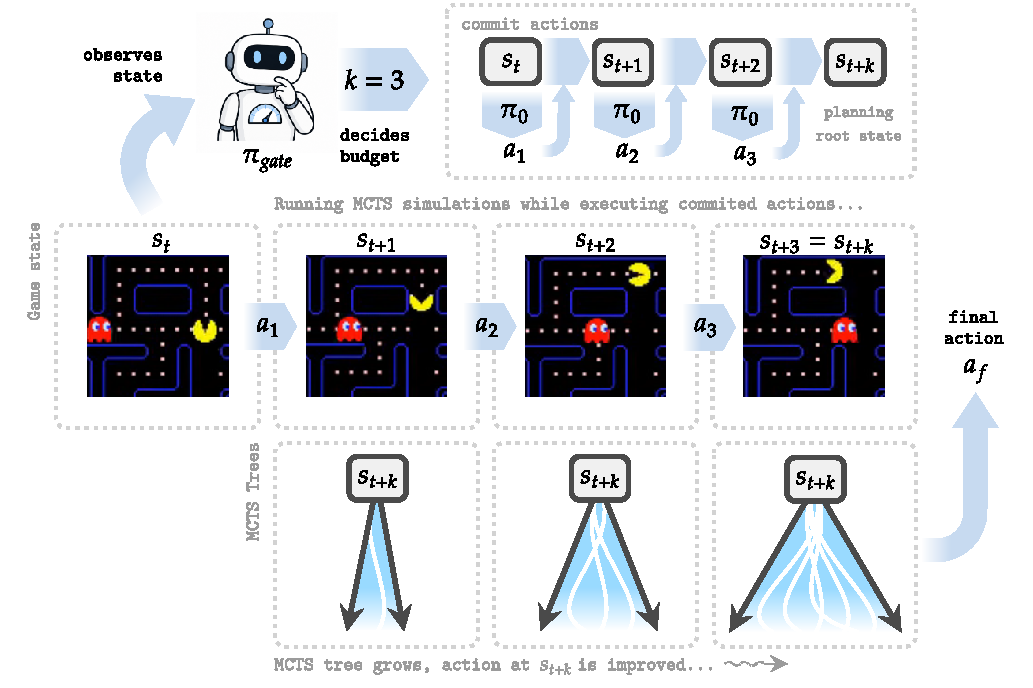
\includegraphics[width=\linewidth]{figures/realtime-rl-gating-diagram.pdf}
  \caption{
    The gating policy chooses whether to react immediately or spend time
    planning.
    Given the current state, a planning budget $K$ is selected, which
    determines how long MCTS runs and, in committed-action environments,
    how many reflex actions are taken.
  }
  \label{fig:realtime-rl-gating-diagram}
\end{figure}

\section{Background and Related Work}
% =============================================================================

\paragraph{Real-time RL and delayed MDPs.}
The standard MDP assumes the environment waits during action selection.
\citet{travnik2018reactive} flagged this as a fundamental mismatch with
real-time interaction, and \citet{ramstedt2019rtrl} formalised an alternative
in which the agent has exactly one timestep to compute its next action,
mathematically equivalent to a 1-step constant-delay
MDP~\citep{walsh2009delayed}.
Subsequent work extends this to fixed action and observation delays of
larger length~\citep{derman2021delayed,bouteiller2021random,katsikopoulos2003markov},
to concurrent control~\citep{xiao2020thinking}, and to asynchronous and
pipelined architectures that mitigate inference cost~\citep{riemer2025staggered,
anokhin2025handling}.
Across this literature, delay is imposed by the system.
We instead let the agent choose its delay $K$ at each decision, turning
delay selection itself into the learning problem.

\paragraph{Value of computation and meta-reasoning.}
The view that rational agents must reason not only about what to do but
about how much to think traces back to bounded
rationality~\citep{simon1955behavioral} and Good's \emph{Type II
rationality}~\citep{good1971twentyseven}.
\citet{russell1991right} made this operational by defining the
\emph{value of computation} (VOC) as the expected improvement in decision
quality minus its cost, and \citet{russell1995provably}'s
bounded-optimality framework reframed rational agency as the optimal use
of fixed computational resources.
Anytime algorithms~\citep{dean1988analysis,zilberstein1996using,
likhachev2003ara,korf1990rta} produce monotonically improving answers as
more time is given, and Bayesian flexible-computation
methods~\citep{horvitz1988reasoning} formalise when to stop.
Applied to MCTS, value-of-computation ideas yield Bayesian formulations
of which simulation to run next~\citep{hay2012selecting,tolpin2012simple,
sezener2020static,lin2015metareasoning}, while classical chess- and
Go-engine time management allocates clock per move via hand-designed
heuristics~\citep{baier2016time,huang2010timemanagement,baudis2012pachi}.
The cognitive-science literature models bounded deliberation itself as a
meta-MDP whose actions are computations~\citep{lieder2017strategy,
griffiths2019doing,callaway2018learning,cope_learning_2023} and shows
empirically that humans allocate planning effort to high-stakes
decisions in ways predicted by this model.
Our gating policy fits this line of work: it is a learned computation
allocator that chooses total budget per decision rather than which
simulation to run next.

\paragraph{Adaptive compute in model-based RL.}
The closest neighbours to our work learn to allocate planning compute on
top of a model-based RL agent.
Metacontrol~\citep{hamrick2017metacontrol} chooses how many imagination
steps to run; Thinker and Dynamic Thinker~\citep{chung2023thinker,
wang2024dynamic} let the agent itself decide when to imagine alternative
trajectories on top of a learned world model; Adaptive
Lookahead~\citep{dalal2022adaptive} learns a state-dependent tree-search
horizon.
\citet{hamrick2021role} provides the key empirical motivation:
shallow MuZero trees often suffice, and the marginal value of additional
simulations varies sharply by state.
AlphaZero-family planners themselves~\citep{silver2018general,
schrittwieser2020muzero,danihelka2022policy} treat MCTS budget as a
fixed deployment hyperparameter.
Our setting differs in two ways: the cost of additional planning is
paid through environmental progression rather than reward shaping, and
the gate operates over a frozen planner rather than being jointly
trained with it.
Other axes of ``learning to search''~\citep{guez2018mctsnets,
farquhar2018treeqn,hamrick2020save,racaniere2017i2a} modify a planner's
internal behaviour rather than its budget; we hold the planner fixed and
control only how long it runs.

\paragraph{Adaptive compute in language models.}
Related ideas have also appeared in sequence models.
PonderNet and adaptive computation time~\citep{graves2016act,
banino2021pondernet,schuster2022calm} learn per-input halting; test-time
compute scaling~\citep{snell2024scaling,deepseek2025r1,muennighoff2025s1}
and RL-trained reasoning-length controllers~\citep{aggarwal2025l1,
muppidi2025predictive,fang2025thinkless,shen2025dast} learn per-query
thinking budgets; cascaded routing~\citep{kim2023bigl,chen2023frugalgpt,
ong2025routellm} defers easy queries to cheap models.
The shared thesis is that a small learned policy can profitably decide
how much computation to spend per decision.
Our setting differs because the cost is endogenous to the environment:
thinking longer changes the state the agent eventually acts in, rather
than merely incurring an external penalty.


% =============================================================================

\section{Variable-Delay Real-Time RL}
\label{sec:envs}
% =============================================================================

This section formalises the variable-delay setting and then describes
the two environment families we study.

\subsection{From fixed to variable action delay}

\citet{ramstedt2019rtrl}'s RTMDP fixes the action delay at exactly one
timestep.
The augmented state $\mathbf{x}_t = (s_t, a_t)$ carries the action
selected at $t{-}1$, and the transition kernel is
\begin{equation}
  p(\mathbf{x}_{t+1} \mid \mathbf{x}_t, \hat{a}_t)
  = p(s_{t+1} \mid s_t, a_t)\,\delta(a_{t+1} - \hat{a}_t),
\end{equation}
which passes the newly emitted action $\hat{a}_t$ forward to land at
frame $t{+}1$.
In RTMDP, delay is a property of the system rather than a choice made by
the agent.

We generalise RTMDP by allowing the action delay to vary per decision.
At each meta-step the gating policy $\pigate$ chooses a budget
$K_t \in \Kset$, and the selected action lands $K_t$ frames later.
Because the environment evolves during those $K_t$ frames, we must also
specify what happens during the $K_t{-}1$ intermediate frames. We call
these filler actions. In committed-action environments they are reflex
actions that move the agent; in clock environments they are no-ops that
consume the player's clock.

Each meta-decision can be viewed as selecting an
\emph{option}~\citep{sutton1999between,bacon2017optioncritic} of length
$K_t$: $K_t{-}1$ filler steps drawn from a fixed reflex distribution,
followed by one action selected by MCTS.
The induced process is a discrete-time semi-Markov decision process
(SMDP) with holding times chosen by the meta-policy, with meta-reward
\begin{equation}
  R_t \;=\; \sum_{k=0}^{K_t - 1} \gamma^k \, r_{t+k}
\end{equation}
and per-meta-step discount $\gamma^{K_t}$, as in the standard options
formulation. The Bellman equation is
\begin{equation}
  V(s_t)
  \;=\;
  \mathbb{E}_{K_t \sim \pigate}\!\left[
    R_t + \gamma^{K_t}\, V(s_{t + K_t})
  \right],
  \label{eq:smdp}
\end{equation}
and we adapt Generalized Advantage Estimation~\citep{schulman2015high}
to carry the per-step discount $\gamma^{K_t}$ through the advantage
computation.
In simulation this is a discrete SMDP with deterministic holding time
set by $K_t$; in deployment, MCTS runtime is slightly stochastic, so
the hardware system is closer to a continuous-time SMDP. Appendix
~\ref{app:rtrl_smdp} discusses this distinction.

Across both environment families, planning is cost-aware by
construction: we do not add a separate reward penalty for thinking.
Either the search tree simulates the effect of delay directly, or the
network is trained on observations that include the remaining time
budget.

\subsection{Committed-action environments: Pac-Man, real-time Tetris, Snake}

In committed-action environments, acting and planning happen
concurrently, and cost-awareness is built directly into the MCTS
search.
When the gating policy selects $K$, it reserves $K$ environment frames
for the planner.
The agent emits $K{-}1$ filler actions---reflex argmax actions drawn
from the planner's own policy network, computed via a single forward
pass in roughly two milliseconds---while the full MCTS runs in the
background.
On the $K$-th frame the planner's chosen action is applied.
The MCTS tree rolls out the same $K{-}1$ reflex steps that the agent
will actually execute, so search is performed over the future state in
which the planned action will land.
The cost of deeper planning is therefore exactly $K{-}1$ additional
frames of world progression before the carefully chosen action lands.

We instantiate this realisation in three environments derived from
Jumanji~\citep{bonnet2024jumanji}: Pac-Man, Snake, and a real-time
variant of Tetris.
The source of progression differs across environments---ghost motion in
Pac-Man, gravity in real-time Tetris, body elongation in Snake---but in
all cases a deeper plan arrives later, after the world has changed.
We modify Jumanji Tetris so that gravity advances the piece in real
time; environment-specific details are in Appendix~\ref{app:envs_tetris}.

\paragraph{Equal compute per frame.}
All budget options in $\Kset$ are calibrated to carry the same number
of MCTS simulations per game frame: at budget $K$ the planner runs
$K \times 32$ simulations over $K$ environment frames, so each frame
receives 32 simulations on average regardless of $K$
(Table~\ref{tab:budget}).
Differences in performance therefore reflect \emph{when} compute is
allocated, not the average compute spent per frame.

\begin{table}[h]
  \centering
  \caption{Committed-action environments: all budget options share 32
    MCTS simulations per game frame.}
  \label{tab:budget}
  \small
  \begin{tabular}{lcccc}
    \toprule
    & $K{=}1$ & $K{=}2$ & $K{=}3$ & $K{=}4$ \\
    \midrule
    MCTS simulations       & 32 & 64 & 96 & 128 \\
    Filler actions         & 0  & 1  & 2  & 3   \\
    Simulations per frame  & 32 & 32 & 32 & 32  \\
    \bottomrule
  \end{tabular}
\end{table}

\subsection{Clock environments: Speed Hex and Speed Go}

In clock environments the board does not evolve while a player
deliberates, but each player has an explicit clock that depletes with
thinking time. Filler actions are no-ops, and only the planner's chosen
action affects the board. Cost-awareness is built into the value
network rather than the search tree: both players' remaining time is
part of the observation during self-play, so the value estimates already
price in the cost of thinking. MCTS can therefore simulate only
board-state dynamics while remaining time-aware through the priors and
values it consumes.
We instantiate this realisation in Speed Hex (11$\times$11) and Speed
Go (9$\times$9), both built on \texttt{pgx}; in both cases the central
decision is not only \emph{which} move to play but \emph{how much} of
the remaining clock to spend before playing it.

\paragraph{Simulation-option calibration.}
For clock environments the equal-compute-per-frame constraint does not
apply, so we calibrate the simulation options $\Kset$ separately to
ensure each option represents a meaningfully distinct tradeoff between
inference latency and planning quality.
Calibration details and the resulting option sets---$\{2,8,32,128\}$
simulations for Speed Hex and $\{16,32,64,96\}$ for Speed Go---are in
Appendix~\ref{app:sim_calibration}.


% =============================================================================

\section{Adaptive Gating Policy}
\label{sec:method}
% =============================================================================

The gating policy is a lightweight network trained on top of a frozen
AlphaZero planner that selects, at each meta-step, a planning budget
$K \in \Kset$.
We described the variable-delay setting it operates in formally in
Section~\ref{sec:envs}; here we describe the policy itself---what it
observes, how it is structured, and how it is trained.

Figure~\ref{fig:scaling} shows the tradeoff the gating policy must
manage: additional MCTS simulations usually improve action quality, but
they also take longer to run.
The planner already handles action selection; the gate only decides,
state by state, how long to run it.
We therefore train the gate on top of a frozen planner rather than
jointly optimizing both components.

\subsection{Observations and architecture}

At each meta-step the gating policy takes three inputs: (1) the raw
game grid, (2) the planner's intermediate spatial features, extracted
from its frozen trunk and used as a compact summary of what the planner
currently infers about the position, and (3) the planner's scalar value
estimate $V(s_t)$.
In clock environments the observation additionally includes the
remaining time budget for both players.
Together these inputs expose the raw state, the planner's internal
representation, and, where applicable, the current time pressure.
We do not feed the planner's policy logits to the gate, so the budget
decision depends on state and planner features rather than directly on
the planner's preferred action.

A lightweight network processes these inputs and produces a categorical
distribution over $K$ together with a scalar baseline value used during
training.
Architecture details, including the recurrent variant used for Speed
Hex, are in Appendix~\ref{app:implementation}.

\subsection{Training}

Training proceeds in two phases.
We first train AlphaZero-style base planners for each environment using
standard expert iteration (Appendix~\ref{app:az_primer}) and select
frozen base checkpoints by cross-evaluation across delay budgets
$K \in \Kset$ (Appendix~\ref{app:cross_eval}).
We then freeze the selected planner and train the gating policy with
PPO~\citep{schulman2017proximal} on top of it.

Rollouts are collected over full episodes. At each meta-step the gate
samples $K_t \sim \pigate(\cdot \mid s_t)$,
the agent executes the resulting option---$K_t{-}1$ filler actions
followed by the planner's chosen action---and the meta-reward $R_t$
defined in Section~\ref{sec:envs} is accumulated.
Variable-duration advantages with per-meta-step discount $\gamma^{K_t}$
are computed before each round of PPO updates, adapting Generalized
Advantage Estimation~\citep{schulman2015high} to the SMDP introduced in
equation~(\ref{eq:smdp}).
Only the gating network is updated; no gradient flows to the planner.

To keep training efficient, we evaluate all $|\Kset|$ option
transitions in parallel at each meta-step.
This preserves static shapes and keeps the training loop easy to
compile.
The full JAX implementation---including the use of \texttt{lax.scan}
for both MCTS inner loops and PPO rollouts, \texttt{vmap} for
environment parallelism, and \texttt{pmap} for device parallelism---is
described in Appendix~\ref{app:implementation}.


\section{Experiments}
\label{sec:experiments}
% =============================================================================

\subsection{Setup}

\paragraph{Environments.}
We evaluate across five environments spanning both mechanisms.
The committed-action group comprises Pac-Man (Jumanji), Real-Time Tetris, and Snake,
each evaluated at simulation budgets of 32, 64, 96, and 128 simulations per move.
The clock group comprises Speed Hex (11$\times$11) and Speed Go (9$\times$9),
with budgets of 2, 8, 32, 128 and 16, 32, 64, 96 respectively.

\paragraph{Baselines.}
For committed-action environments we compare against \emph{always-$K$}
policies for each $K \in \Kset$ and a \emph{random} policy that samples
$K$ uniformly at each meta-step. For clock environments we additionally
compare against \emph{greedy} (always use the maximum simulation
budget) and \emph{midpeak} (a bell-curve schedule that concentrates
compute in the midgame, following common game-engine practice
\cite{baier2016time, huang2010timemanagement}). We tune the midpeak
shape separately at each evaluation budget and report the best result.

\paragraph{Base planner.}
For committed-action environments we use an AlphaZero checkpoint trained without
action delay ($K{=}1$) as the frozen base.
Cross-evaluation across checkpoints trained at each $K$ shows this checkpoint
is best overall (Appendix~\ref{app:cross_eval}).

\paragraph{Evaluation protocol.}
All results are averaged over 100 independent episode seeds; we report mean $\pm$ standard error.

\subsection{Main results}

\begin{figure}[t]
  \centering
  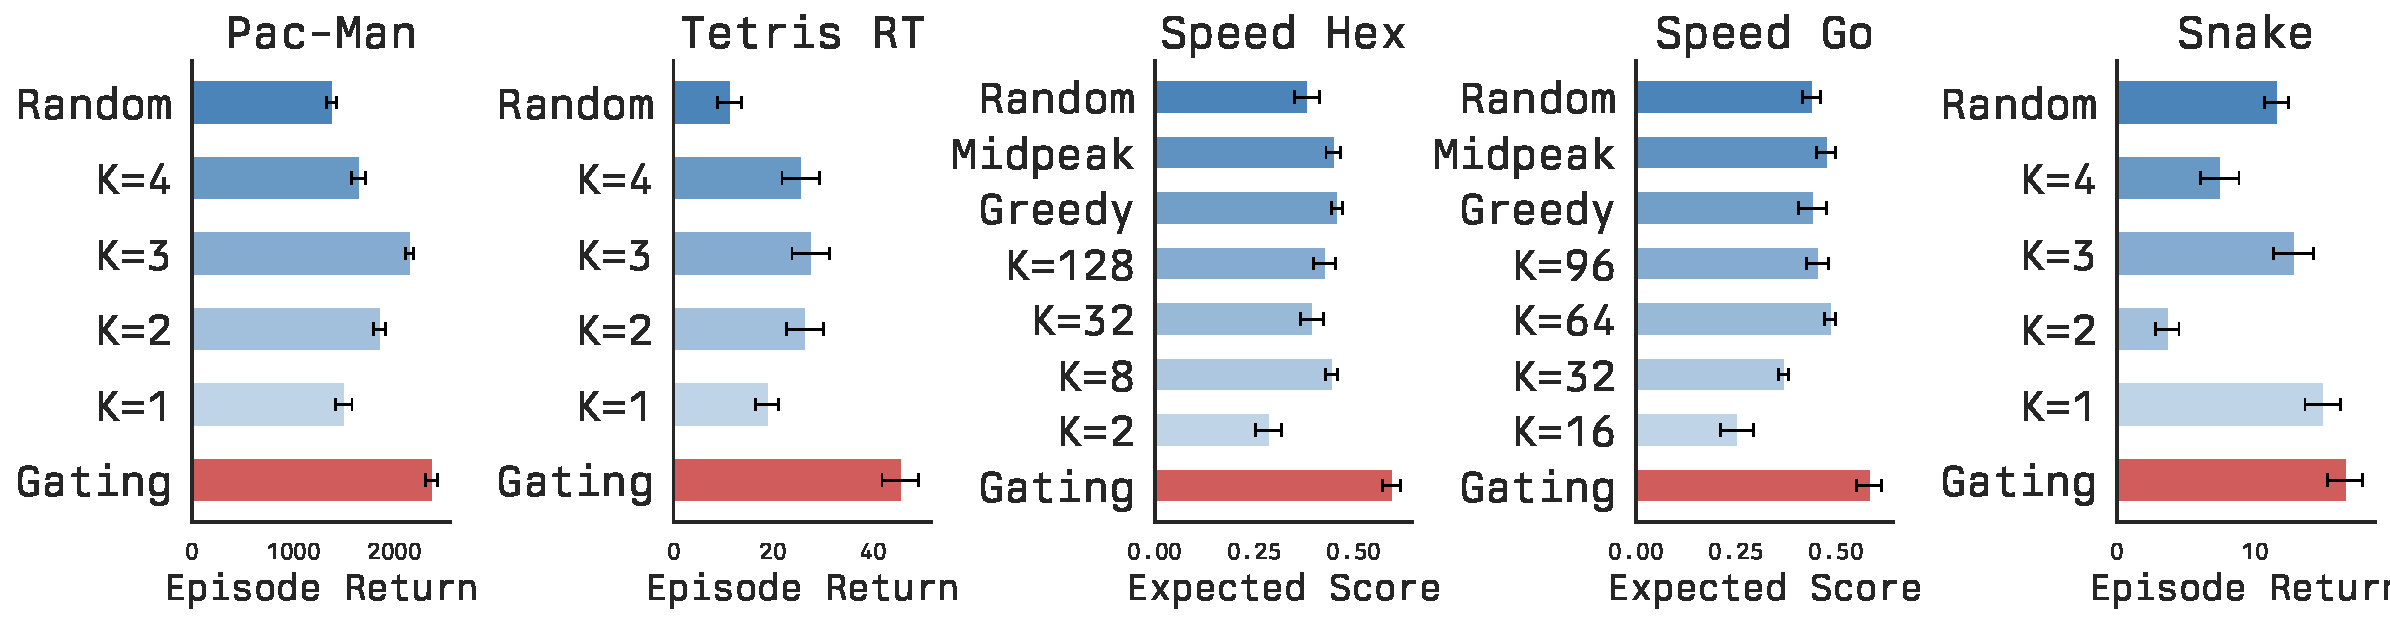
\includegraphics[width=\linewidth]{figures/main_results_horizontal.pdf}
  \caption{
    Across all five environments, the gating policy outperforms fixed-budget and
    heuristic baselines, showing that adaptive allocation matters more than
    committing to a single search budget. Bars show mean $\pm$\,SE over 100
    episodes; for Speed Hex and Speed Go, expected score is averaged over the
    shared sampled clock budgets.}
  \label{fig:main_results}
\end{figure}

The gating policy outperforms every fixed-budget baseline across all
five environments. In Pac-Man, the best fixed policy ($K{=}3$, 96
simulations per step) scores 2149, while the gate reaches 2370
($+10.3\%$) using about 49 simulations per frame on average. In
real-time Tetris, the best fixed policy ($K{=}3$) scores 27.6, while
the gate reaches 45.6 ($+65\%$). In Snake, the best fixed policy
($K{=}1$) scores 14.91, while the gate reaches 16.54 ($+10.9\%$) by
mostly reacting quickly and invoking deeper planning selectively.

For Speed Hex and Speed Go, we evaluate each policy at five sampled
clock budgets, $T \in \{300, 1200, 2300, 3500, 4800\}$, and average the
resulting head-to-head expected scores. Here $K{=}1,\dots,4$ denotes
the four simulation-budget options rather than committed-action lengths:
2/8/32/128 simulations for Speed Hex and 16/32/64/96 for Speed Go.
Against fixed-budget baselines and the greedy, midpeak, and random
heuristics, the gating policy remains above parity on average and
outperforms all of them overall.

Across environments, the learned gate does not collapse to a single
budget. It learns state- and budget-dependent allocation strategies
that beat both fixed policies and hand-designed heuristics
(Figure~\ref{fig:strategy}, Appendix Figure~\ref{fig:strategy_appendix}).
The random baseline falls well below every fixed-$K$ policy, confirming
that \emph{when} compute is allocated matters as much as how much.

\subsection{What triggers deeper planning?}

Across environments, the gate allocates more compute in higher-stakes
states, where a poor action is costly and extra search is more likely
to change the decision.

\paragraph{Pac-Man}

Ghost proximity correlates with lower chosen budgets in Pac-Man: the
policy prefers $K{=}1$ when the nearest ghost is far away, shifts
toward $K{=}2$ as the threat closes in, and reaches for $K{=}4$ at
extreme proximity. When ghosts are frightened, the policy reduces the
budget again.

\paragraph{Tetris}

Board density is the dominant feature in Tetris.
$K{=}1$ is selected almost exclusively on near-empty boards
(fill $\approx 0.05$, stack $\approx 3.5$ rows) where any reasonable placement is
acceptable.
$K{=}2$ and $K{=}4$ are selected on dense boards (fill
$\approx 0.25$--$0.32$, stacks $\approx 12$ rows) where placement
precision matters.
$K{=}3$ is never used ($0\%$), producing the bimodal ``react or plan deeply'' strategy
visible in Figure~\ref{fig:strategy}.
Piece type also modulates budget: the Z-piece ($\bar{K}{=}2.98{\scriptstyle\pm0.04}$)
and O- and T-pieces ($\bar{K}{=}2.88{\scriptstyle\pm0.04}$) receive the most
deliberation, while the J-piece ($\bar{K}{=}2.66{\scriptstyle\pm0.04}$) receives the
least, reflecting differences in placement geometry and expected outcome variance.

\paragraph{Snake}

Spatial constraint, rather than simple goal distance, is the main
trigger.
$K{=}1$ dominates on open boards, while $K{=}3$ appears when reachability drops,
local body density rises, and the snake has fewer safe continuations. $K{=}2$
occupies a milder regime associated with navigating toward more distant fruit on
otherwise open boards. Immediately after eating, when the body has just grown,
$K{=}3$ usage jumps from $3.2\%$ to $13.5\%$, indicating that the policy treats
body-growth events as a prospective spatial-risk signal.

\paragraph{Clock environments}

In the clocked PGX games, the relevant signal is the interaction
between board state and remaining time. Figure~\ref{fig:strategy} shows
that under the small clock budget ($T{=}300$), the policy heavily
favours the cheapest option, while under the larger budget
($T{=}4100$), it spreads mass more evenly across the four choices and
uses deeper search more often. Because the policy is trained across many
clock settings rather than tuned separately at each one, this shift is
evidence of budget-conditioned generalization. A strict-timeout Speed
Hex control in Appendix~\ref{app:hex_timeout_control} shows why we do
not use that variant as the main clock benchmark: once running out of
time becomes an immediate loss with no fallback, the task becomes much
easier and the main challenge is simply avoiding flag-falls.
Appendix~\ref{app:strategy_appendix} shows the full per-environment
strategy plots.

\begin{figure}[t]
  \centering
  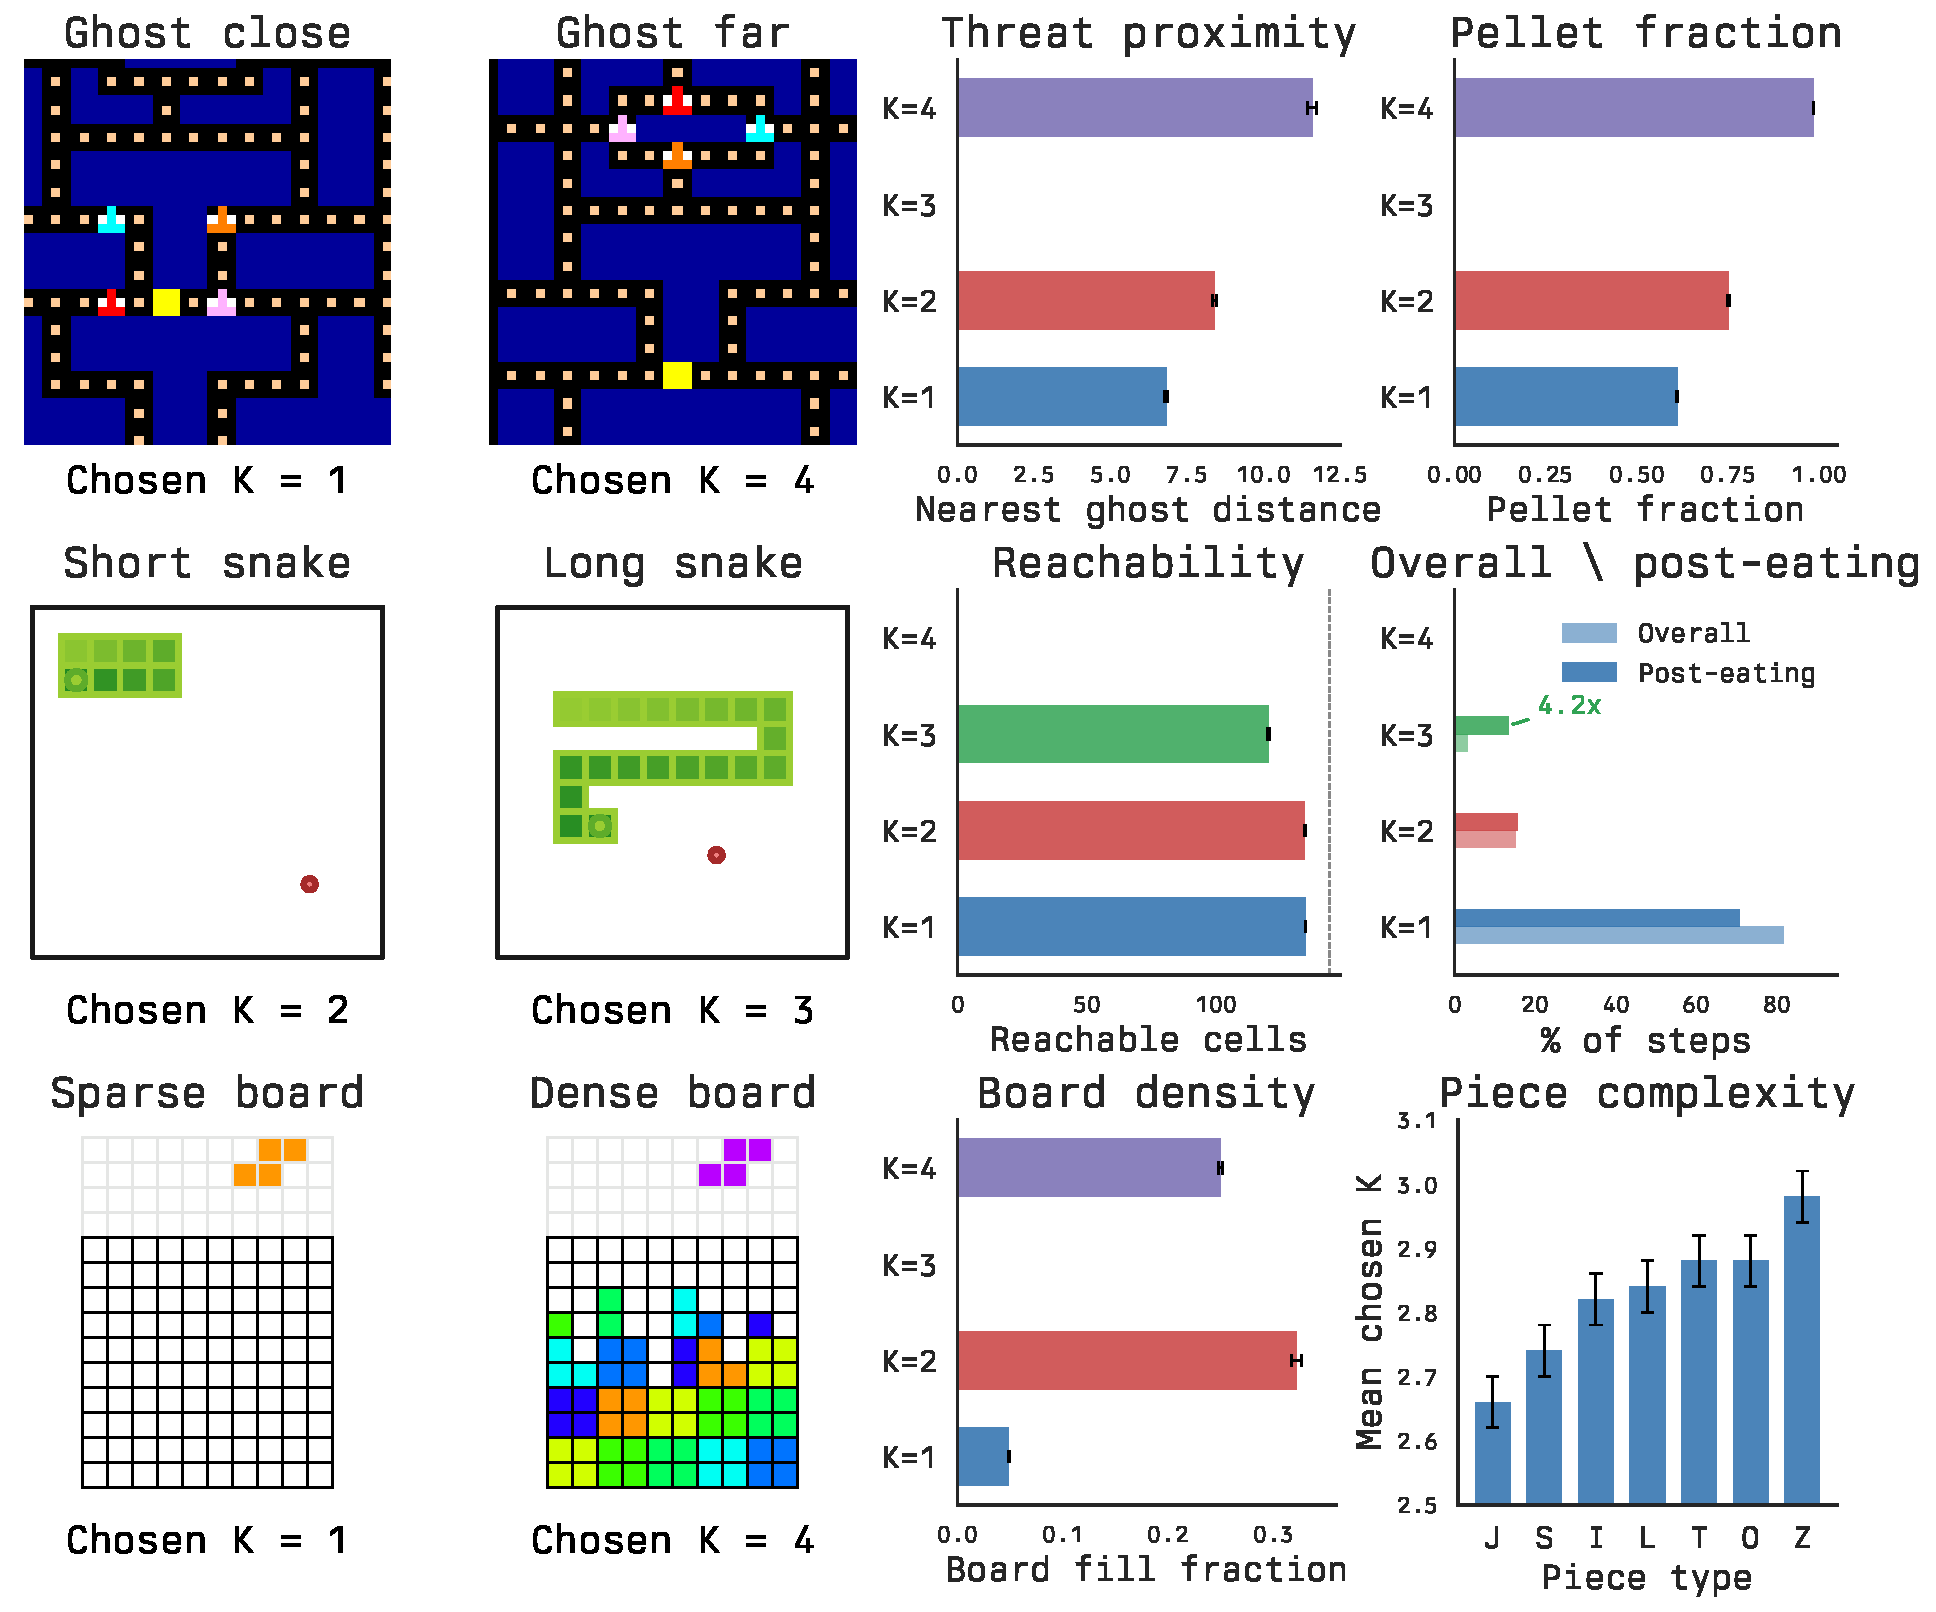
\includegraphics[width=\linewidth]{figures/interpretability_combined_alt.pdf}
  \caption{The policy plans deeply precisely when the state is dangerous or constrained.
    Across Pac-Man, Tetris, and Snake, larger chosen budgets are associated with
    higher threat, denser boards, or fewer safe continuations, indicating that
    the gate is responding to meaningful decision difficulty. Plots show state
    features conditioned on chosen budget $K$ (mean $\pm$\,1\,SE, 100 episodes).}
  \label{fig:interpretability}
\end{figure}



\begin{figure}[t]
  \centering
  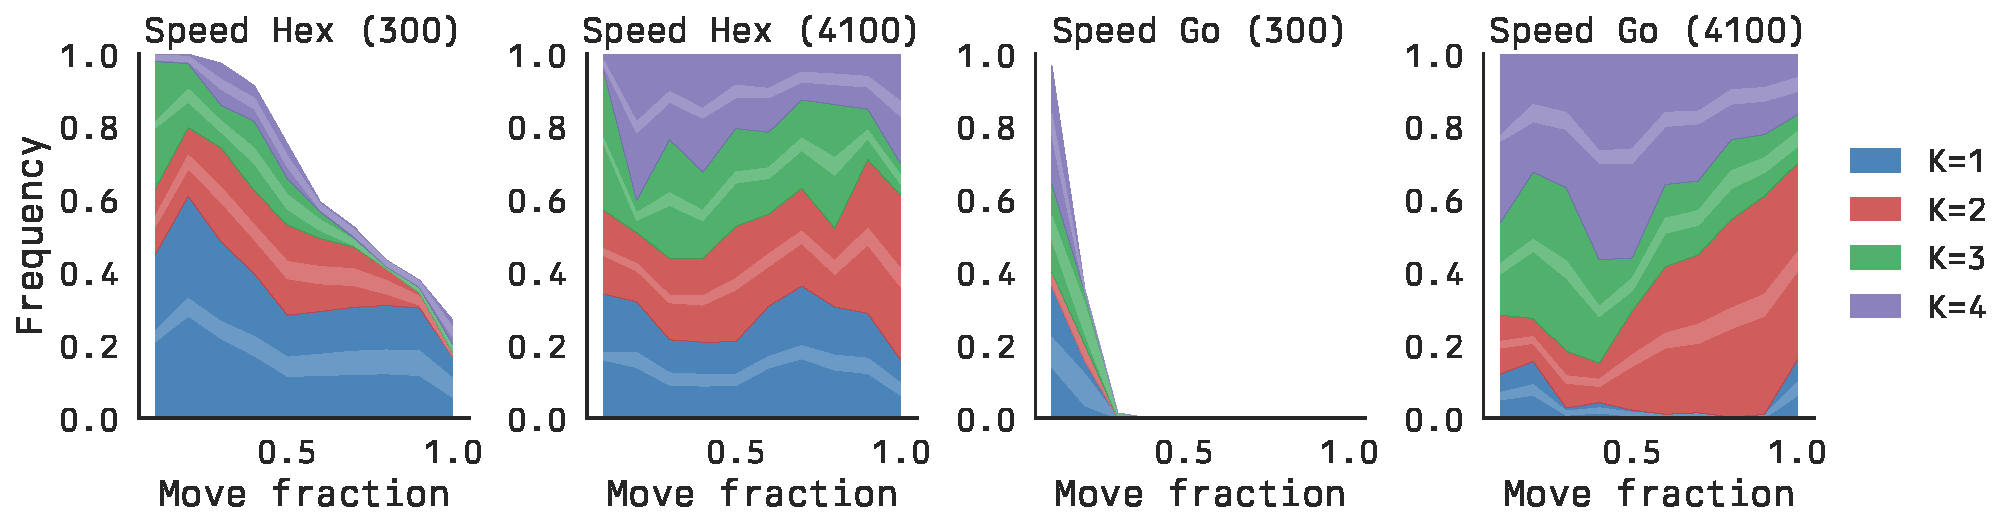
\includegraphics[width=1\linewidth]{figures/strategy_band.pdf}
  \caption{ In both Speed Hex and
    Speed Go, the learned policy is much more reactive under the small budget
    ($T{=}300$) and distributes mass toward deeper options once more clock is
    available ($T{=}4100$).}
  \label{fig:strategy}
\end{figure}


% =============================================================================

\section{Real-Time Deployment}
\label{sec:deployment}
% =============================================================================

We validate the committed-action framework in a two-GPU real-time setup
across real-time Tetris, Pac-Man, and Snake. One GPU runs the
environment and executes committed actions continuously; the second runs
MCTS. At each meta-decision the current game state is transferred to
the planning GPU, which searches while the environment GPU keeps the
game moving. When planning finishes, after $K \times 32$ simulations,
the resulting action is applied at the next environment step
(Figure~\ref{fig:deployment_timeline}).

Figure~\ref{fig:deployment} summarizes 45 measured deployments:
3 environments $\times$ 3 GPU classes $\times$ 5 frame rates (8--12\,FPS).
The asynchronous execution pattern is unchanged from training: a $K{=}4$
meta-step at 9\,FPS spans four 111\,ms frames, while reflex actions keep the
environment moving and MCTS finishes asynchronously on the second GPU.

The main result is that simulation-trained policies transfer cleanly to
asynchronous hardware deployment over a broad operating range. Latency
stays within budget on H100 in all three environments, and remains
reliable on A100 except near the tightest deadlines. Return transfer is
also strong: at 9\,FPS, deployed returns remain close to their
simulation counterparts, and the learned budget distribution carries
over as well. In Tetris on H100, the deployed policy preserves the same
strongly bimodal ``react or plan deeply'' strategy seen in simulation.
Appendix~\ref{app:deployment_details} gives the full breakdown by
environment, FPS, and GPU.

This result validates the committed-action training protocol. Because
training already simulates planning delay by executing committed
actions, the learned policy transfers to asynchronous deployment
without modification. A fixed 1-step RTMDP formulation
~\citep{ramstedt2019rtrl} is not expressive enough for variable-budget
MCTS spanning $K \in \{1,\ldots,4\}$ frames; a naive extension would
need to carry a variable number of stale actions in the state. Appendix
~\ref{app:rtrl_smdp} discusses this point in more detail.

\begin{figure}[h]
  \centering
  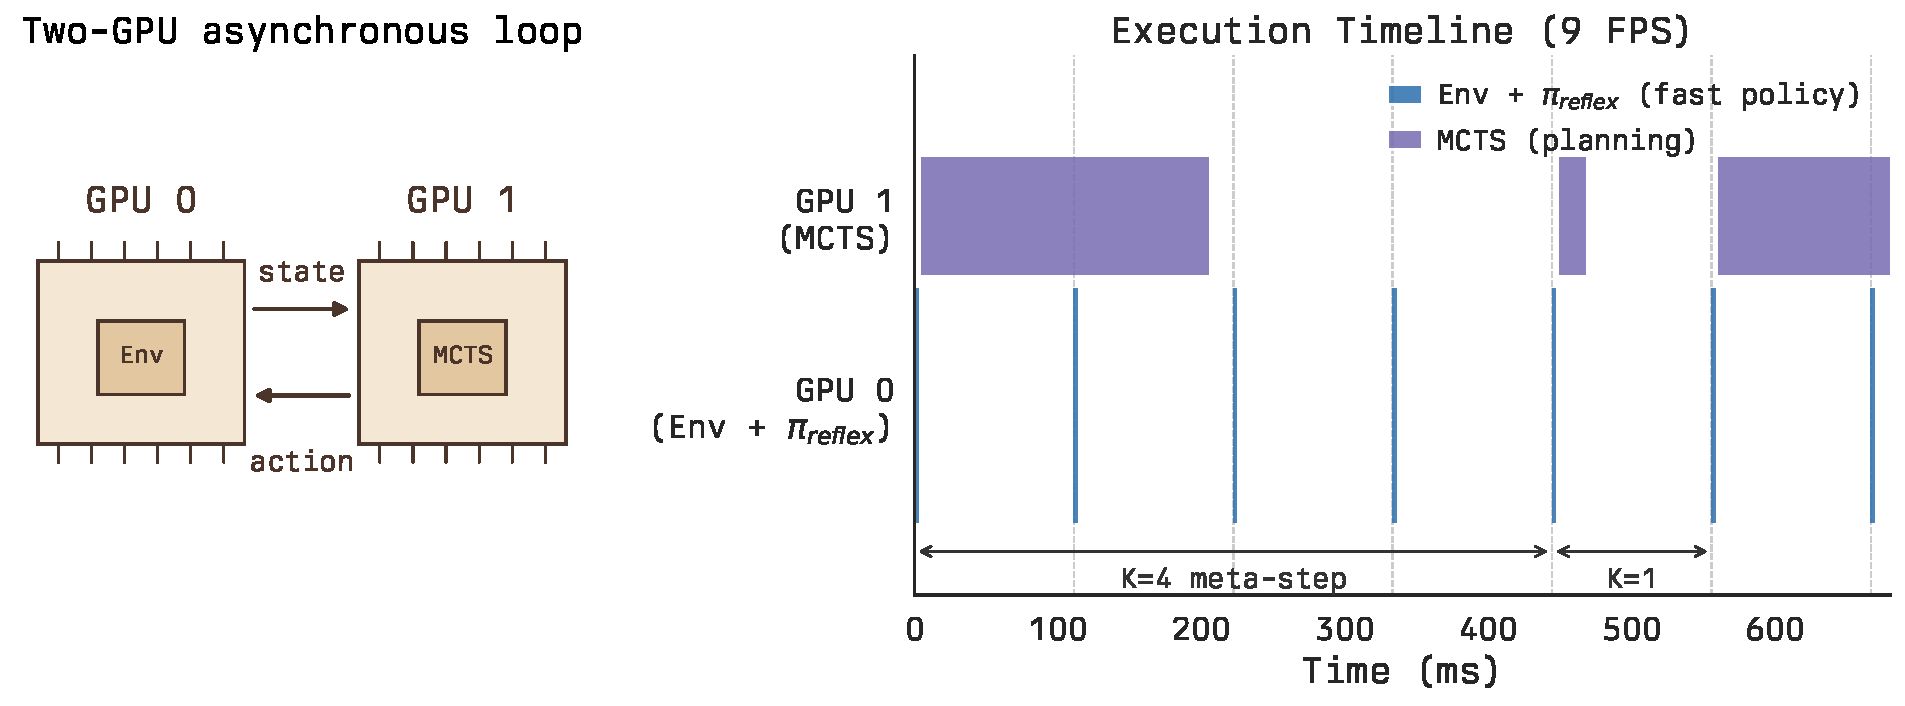
\includegraphics[width=\linewidth]{figures/deployment_timeline.pdf}
  \caption{\textbf{Two-GPU real-time deployment pipeline.}
    GPU~0 runs the environment continuously via committed (reflex) actions;
    GPU~1 runs MCTS in parallel, so a larger $K$ buys more planning time without
    pausing the game.
    \emph{Left:} schematic of the two-GPU loop.
    \emph{Right:} execution trace at 9\,FPS---a $K{=}4$ meta-step spans four 111\,ms
    frames, followed by a $K{=}1$ recovery step.}
  \label{fig:deployment_timeline}
\end{figure}

\begin{figure}[h]
  \centering
  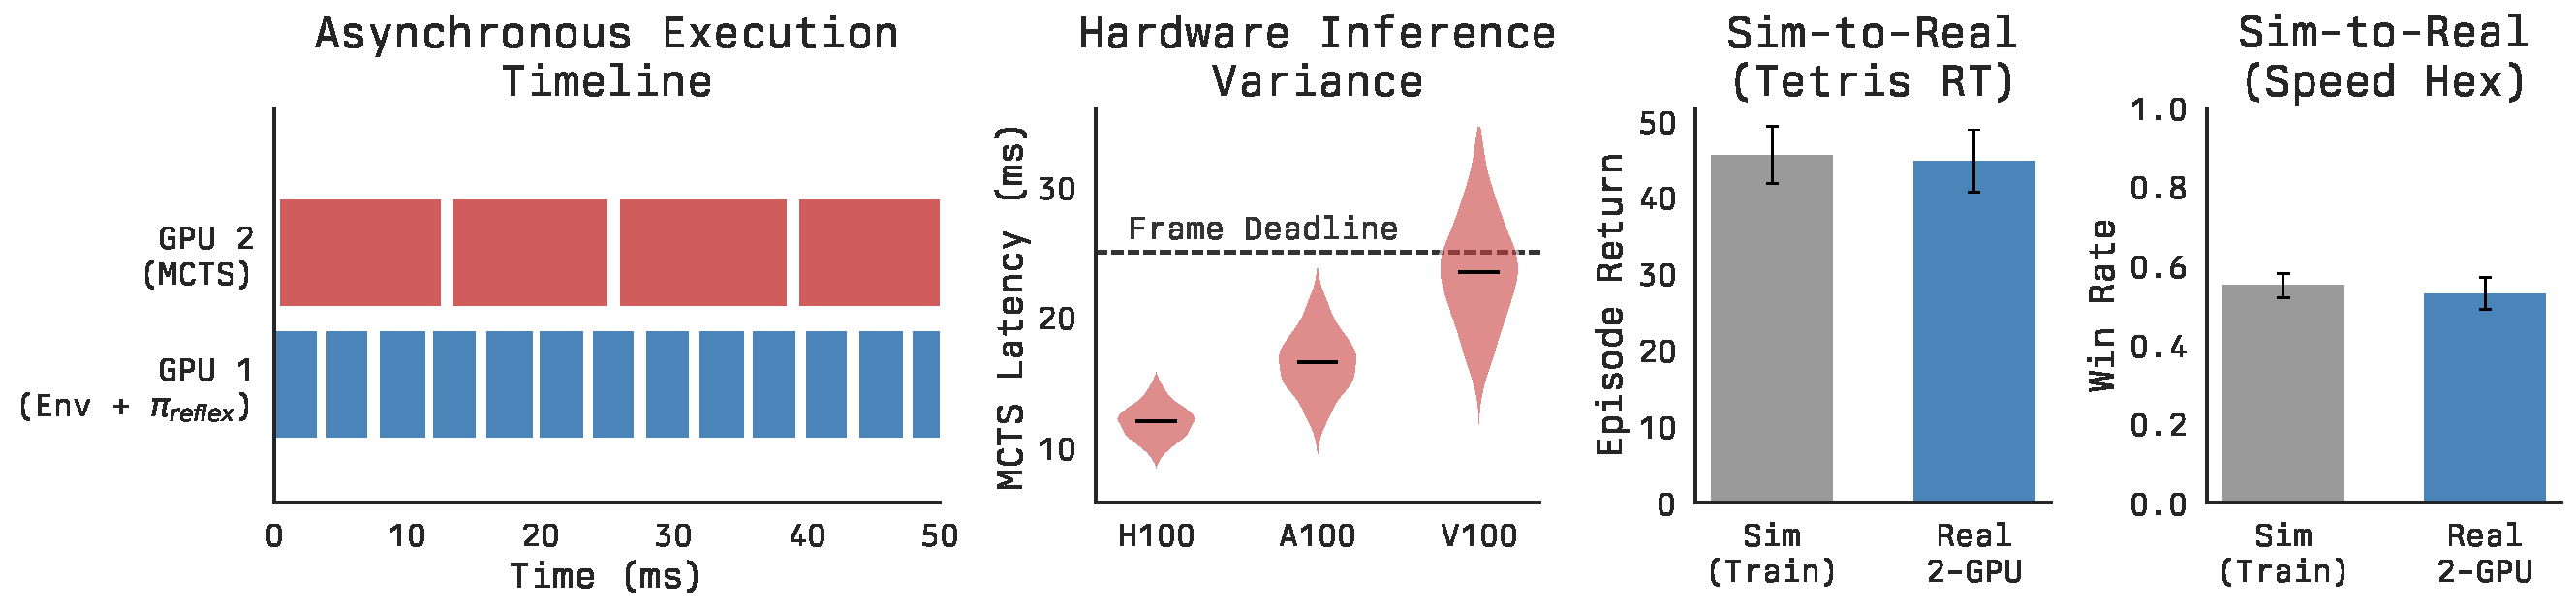
\includegraphics[width=\linewidth]{figures/deployment.pdf}
  \caption{\textbf{Simulation-trained policies transfer cleanly to hardware deployment.}
    \emph{Left:} MCTS latency variance tightens with GPU class---H100 is most
    consistent, A100 intermediate, A40 widest.
    \emph{Centre:} H100 and A100 miss deadlines rarely; A40 breaks down only at
    the tightest frame rates.
    \emph{Right:} Deployed returns at 9\,FPS match simulation closely across all
    environments and GPU classes.
    See Appendix~\ref{app:deployment_details} for the full breakdown.}
  \label{fig:deployment}
\end{figure}

% =============================================================================

\section{Discussion}
% =============================================================================


\paragraph{A unified framework.}
The committed-action and clock mechanisms are two realizations of the
same principle: planning should be cost-aware by construction. In
committed-action environments, cost-awareness is built into the MCTS
tree, which searches over the future state induced by planning delay. In
clock environments, it is built into the value function, which is
trained on clock-augmented observations.
The gating policy can exploit both signals using the same learning algorithm.

\paragraph{Deployment as a test of training fidelity.}
The two-GPU deployment result is not just an engineering demonstration.
It shows that the committed-action abstraction, in which $K{-}1$ reflex
actions fill the planning delay during training, is a good model of
true asynchronous execution. An agent trained under this abstraction
transfers directly to hardware-separated deployment.

\paragraph{Limitations.}
The gating policy is trained on top of a fixed base planner, so joint
optimization remains open. We also study a discrete budget set
$K \in \Kset$; richer compute vocabularies, and eventually continuous
allocation, are natural extensions. Finally, our environments are
either simulated or played at controlled speeds; physical real-time
settings with uncontrolled latency would require adaptive calibration of
the timing model.


% =============================================================================
\section{Conclusion}
% =============================================================================

We studied planning in real-time reinforcement learning, where the cost
of deliberation is paid through game outcomes rather than wall-clock
seconds alone. A lightweight gating policy trained on top of a frozen
planner learns to allocate computation by state, spending more on
constrained or high-stakes decisions and less on easy ones. Across five
environments spanning two real-time mechanisms, this policy
consistently beats fixed-budget baselines while often using less
average compute. Adaptive, state-conditioned compute allocation is a
practical way to make planning-based RL systems more capable and more
efficient in real-time settings.


\begin{ack}
\todo{Acknowledgments, funding disclosure, and competing interests.}
\end{ack}


% =============================================================================
% =============================================================================

\bibliographystyle{plainnat}
\bibliography{refs}


%%%%%%%%%%%%%%%%%%%%%%%%%%%%%%%%%%%%%%%%%%%%%%%%%%%%%%%%%%%%

\appendix

\section{AlphaZero and MCTS}
\label{app:az_primer}

This section answers common questions about the planning infrastructure used in this
paper. It targets readers familiar with deep RL but not with tree-search methods.

\textbf{What does ``running a simulation'' mean in MCTS?}

A \emph{simulation} (also called a \emph{playout}) is one traversal of the search tree
from the root node (the current observed state) to a leaf, followed by a backup of
the resulting value estimate up to the root.
Each traversal selects edges greedily according to the PUCT rule:
\[
  a^* = \arg\max_a \Bigl[Q(s,a)
        + c \cdot \pi_\theta(a|s)
          \cdot \frac{\sqrt{N(s)}}{1+N(s,a)}\Bigr],
\]
where $Q(s,a)$ is the empirical mean value of subtree $a$,
$\pi_\theta(a|s)$ is the network's prior over actions,
$N(s)$ is the total visit count of node $s$,
and $N(s,a)$ is the visit count of edge $(s,a)$.
Repeated simulations concentrate visits on high-value, high-prior subtrees while
continuing to explore less-visited ones.
After $n$ simulations the recommended action is the \emph{most-visited} child of
the root.

\textbf{How is the final action selected?}

At evaluation time the agent picks the most-visited root child.
During training, the visit-count distribution
$\hat{\pi}(a) \propto N(s_0,a)^{1/\tau}$
(temperature $\tau > 0$) is recorded and used as a \emph{search target}:
the network is updated to predict $\hat{\pi}$ at state $s_0$.
This is the expert-iteration loop as search produces a better-than-raw-policy
distribution, and the network learns to imitate it, improving its prior for
future searches.


\textbf{What is the difference between AlphaZero and MuZero?}

\textbf{AlphaZero}~\cite{silver2018general} requires a \emph{perfect simulator}:
given state $s$ and action $a$, the simulator returns the exact next state $s'$.
MCTS is run entirely inside this simulator; the network supplies priors and value
estimates but never models transitions.

\textbf{MuZero}~\cite{schrittwieser2020muzero} replaces the perfect simulator with a
\emph{learned latent-space dynamics model}.
Transitions during search are predicted by a network rather than a ground-truth
engine, so MuZero can plan in environments without a simulator (e.g.\ Atari frames).

All environments in this paper expose a JAX-native step function, so we use the
AlphaZero paradigm: ground-truth transitions, no learned dynamics.

\textbf{AlphaZero was designed for two-player zero-sum games. How does it transfer to single-agent settings?}

The core loop is \emph{expert iteration}~\cite{anthony2021expert},
shown in Algorithm~\ref{alg:expert_iter}.
The value head uses a bootstrapped return instead of a zero-sum game outcome;
otherwise the algorithm is identical to two-player AlphaZero.

\begin{algorithm}[h]
\caption{Single-agent AlphaZero via Expert Iteration}
\label{alg:expert_iter}
\begin{algorithmic}[1]
\Require Network $f_\theta = (\pi_\theta, v_\theta)$, environment $\mathcal{E}$,
         simulations per step $n$, replay buffer $\mathcal{B}$
\Repeat
  \State $\mathcal{D} \leftarrow \{\}$ \Comment{episode data buffer}
  \State $s_0 \leftarrow \mathcal{E}.\text{reset}()$
  \For{$t = 0, 1, \ldots, T-1$}                     \Comment{\textbf{Act}}
    \State Run $n$ MCTS simulations from $s_t$ using $f_\theta$
    \State $\hat{\pi}_t(a) \propto N(s_t, a)^{1/\tau}$ \Comment{visit-count policy}
    \State $a_t \sim \hat{\pi}_t$;\quad $s_{t+1} \leftarrow \mathcal{E}.\text{step}(a_t)$
    \State $\mathcal{D} \leftarrow \mathcal{D} \cup \{(s_t,\, \hat{\pi}_t)\}$
  \EndFor
  \State Compute returns $z_t = \sum_{k \geq 0} \gamma^k r_{t+k}$ for each $t$ \Comment{\textbf{Store}}
  \State $\mathcal{B} \leftarrow \mathcal{B} \cup \{(s_t, \hat{\pi}_t, z_t)\}_{t=0}^{T-1}$
  \State Sample mini-batch from $\mathcal{B}$                     \Comment{\textbf{Learn}}
  \State $\mathcal{L}(\theta) =
    \displaystyle\frac{1}{|\mathcal{B}|}\sum_{(s,\hat{\pi},z)\in\mathcal{B}}
    \Bigl[\bigl(v_\theta(s) - z\bigr)^2
          - \hat{\pi}^\top \log \pi_\theta(s)\Bigr]$
  \State $\theta \leftarrow \theta - \alpha\,\nabla_\theta\,\mathcal{L}(\theta)$
\Until{convergence}
\end{algorithmic}
\end{algorithm}


\textbf{MCTS sounds inherently sequential. How do you run it efficiently at the scale needed for RL training?}

Naively each MCTS simulation depends on the previous one (via the updated $Q$ and $N$
tables), which conflicts with JAX's strength: massive data-parallel operations.
We exploit two levels of parallelism.

\textbf{Environment-level parallelism.}
We maintain a batch of $E$ independent environment instances (32 in our experiments).
Each instance has its own search tree; all $E$ leaf nodes are evaluated in a
\emph{single batched forward pass} of the neural network, which is the GPU/TPU
bottleneck.

\textbf{Intra-tree simulation loop via \texttt{jax.lax.scan}.}
Within each tree the $n$ simulations are unrolled as a \texttt{scan}.
Each iteration: (1) traverse all $E$ trees to their current leaf using PUCT
(parallelised over $E$), (2) batch-evaluate the $E$ leaves in one network call,
(3) back-propagate values.
Because JAX traces the full scan at compile time, the tree-update logic is fused
into a single XLA kernel with zero Python-level iteration overhead at runtime.

The result is that all $n$ simulations across all $E$ environments are compiled
into a single \texttt{jit}-ted function that runs entirely on the accelerator,
with one network forward pass per simulation step and no host-device transfers
during rollout.


\section{Environment Details}
\label{app:envs}

\subsection{Real-time Tetris}
\label{app:envs_tetris}

Our real-time Tetris environment is a modification of Jumanji Tetris in which each
environment step is one gravity tick rather than one full placement decision.
The board is $20 \times 10$, episodes last at most 2000 gravity ticks, and the
observation contains the locked board, the current falling tetromino, its
$(x,y)$ position, and the gravity-tick count.

Every call to \texttt{env.step(action)} first applies the chosen control and then
applies one gravity update. The action set has six elements:
\begin{itemize}[nosep]
  \item \textbf{Left / Right}: translate the falling piece one column in the respective
    direction; invalid lateral moves are ignored.
  \item \textbf{Rotate-CW / Rotate-CCW}: rotate the piece $90°$ clockwise or
    counter-clockwise; invalid rotations are ignored.
  \item \textbf{Hard-drop}: instantly translate the piece to the lowest valid row and
    lock it; a new piece spawns immediately.
  \item \textbf{Noop}: no horizontal or rotational change; the piece descends one row
    by gravity.
\end{itemize}
A piece also locks whenever gravity would move it into an occupied cell; completed
rows are then cleared and scored with the standard convex Tetris reward schedule.
The episode ends on board top-out, i.e.\ when a newly spawned piece cannot be placed
at the spawn position, or when the 2000-tick horizon is reached.

For the committed-action experiments in the main paper we use the \texttt{TetrisRTKT}
variant. The underlying environment dynamics are identical, but during the $K{-}1$
delay steps inside MCTS the tree rolls out policy-guided committed actions rather
than assuming a pure gravity-only noop sequence. This makes the search-time delay
model match the deployment-time reflex behavior more closely.

\subsection{Committed-action execution}
\label{app:committed_action}

During the $K{-}1$ delay steps while the MCTS planner is running, the agent executes
committed actions in the environment.
In all variants these are drawn from the argmax of the base model's raw policy
logits---a single inexpensive forward pass, with no additional MCTS compute.
The two variants differ only in what the \emph{MCTS tree simulates} during its internal
rollout of the delay window, not in what is executed in the environment.

\textbf{RT\_KStep (noop)} simulates the delay steps inside the tree using a fixed
action (gravity/noop), which is fast but mismatches what the agent will actually do.

\textbf{RT\_KT (logit)} simulates the delay steps inside the tree using
$\mathrm{argmax}(\pi_{\mathrm{logits}})$, matching the committed actions the agent
executes at deployment and making the search model more accurate at no extra
environment cost.
All Tetris results reported in the main paper use the RT\_KT variant.

Crucially, neither variant uses MCTS for the committed actions executed in the
environment, so there is no compute-parity violation: every option $K \in \Kset$
uses the same number of policy forward passes for its delay steps.

\subsection{Speed Hex}
Speed Hex is built on the pgx Hex library (11$\times$11 board).
Each player begins with $T = 300$ clock ticks; time spent planning is deducted after
each move.
MCTS search uses board-only dynamics (no clock deduction during simulation), but the
observation (and therefore the network's value estimates) includes the remaining
clock for both players.
The gating policy is a GRU network that maintains hidden state across moves within an
episode, allowing it to track game progression and clock pressure jointly.

\paragraph{Training notes.}
Early experiments fine-tuned the gating policy against fixed-budget opponents rather
than via self-play.
This regime exhibited plasticity loss, the network's ability to adapt to new opponents
degraded over successive fine-tuning rounds, consistent with findings in continual RL
settings~\citep{muppidi2024fast, boopathy2024permutation}.
We therefore switched to self-play, which eliminated plasticity loss entirely.
In self-play we found that increasing entropy regularization was the single most
impactful training intervention, consistent with recent results in other self-play
board-game domains~\citep{forkel2025entropy}.

\subsection{Speed Go}
Speed Go is built on the pgx Go library (9$\times$9 board).
As in Speed Hex, each player has an explicit clock, planning consumes clock only
after the move is played, and MCTS search itself uses board-only dynamics while the
network observes the remaining clock for both players.
We use the same recurrent gating architecture and evaluate the policy over the same
shared five sampled clock budgets used in the main text.
The same training observations apply: self-play with elevated entropy regularization
was decisive, and no plasticity loss was observed once fine-tuning against fixed
opponents was abandoned.


\section{Simulation Option Calibration for Clock Environments}
\label{app:sim_calibration}

For committed-action environments, the equal-budget constraint (32 sims/frame) naturally
produces meaningful option spacing.
For clock environments this constraint does not apply, so we select simulation options
by examining two curves simultaneously: planning quality (win rate or return) vs.\
simulation count, and inference latency vs.\ simulation count.

An option is \emph{useful} if it is distinguishable from its neighbors on both dimensions:
adding more simulations should noticeably improve play \emph{and} noticeably increase
latency.
Options that are close in both cost and quality give the gating policy nothing to learn;
options that differ in cost but not quality waste planning budget.

For Speed Hex we found that options $\{2, 8, 32, 128\}$ satisfy this criterion across
the relevant range of clock settings, and for Speed Go we found that
$\{16, 32, 64, 96\}$ yield similarly distinct quality-latency tradeoffs.
Figure~\ref{fig:scaling_appendix} shows the full co-scaling results across all five
evaluation environments.

\paragraph{Go and Hex calibration.}
To calibrate the clock-environment options more directly, we examine how average
expected score changes as inference budget increases.
The resulting curves are shown in Figure~\ref{fig:clock_budget_calibration}.
For Speed Go, the selected set $\{16, 32, 64, 96\}$ spans the steep part of the
quality curve: average expected score versus all other budgets rises from $0.314$
at 16 simulations to $0.506$ at 32, $0.704$ at 64, and $0.782$ at 96.
The largest gains occur at $16{\rightarrow}32$ ($+0.193$) and
$32{\rightarrow}64$ ($+0.198$), while $64{\rightarrow}96$ still provides a clear
additional improvement ($+0.078$).
Pairwise tournament results among the selected Go options also remain well
separated: 64 simulations scores $0.713$ against 32 and $0.868$ against 16,
while 96 scores $0.595$ against 64 and $0.773$ against 32.

For Speed Hex, the selected set $\{2, 8, 32, 128\}$ follows the same design
principle and is now supported by the completed inference-budget tournament.
Average expected score versus all other budgets rises from $0.340$ at 2
simulations to $0.422$ at 8, $0.495$ at 32, and $0.710$ at 128, with successive
gains of $+0.082$, $+0.073$, and $+0.214$.
The pairwise Hex tournament shows the same separation: 8 simulations scores
$0.550$ against 2, 32 scores $0.564$ against 8 and $0.643$ against 2, and 128
scores $0.693$ against 32 and $0.727$ against 8.
Thus, in both clocked domains, the selected options provide the
gating policy with meaningfully separated quality-latency tradeoffs.

\begin{figure}[h]
  \centering
  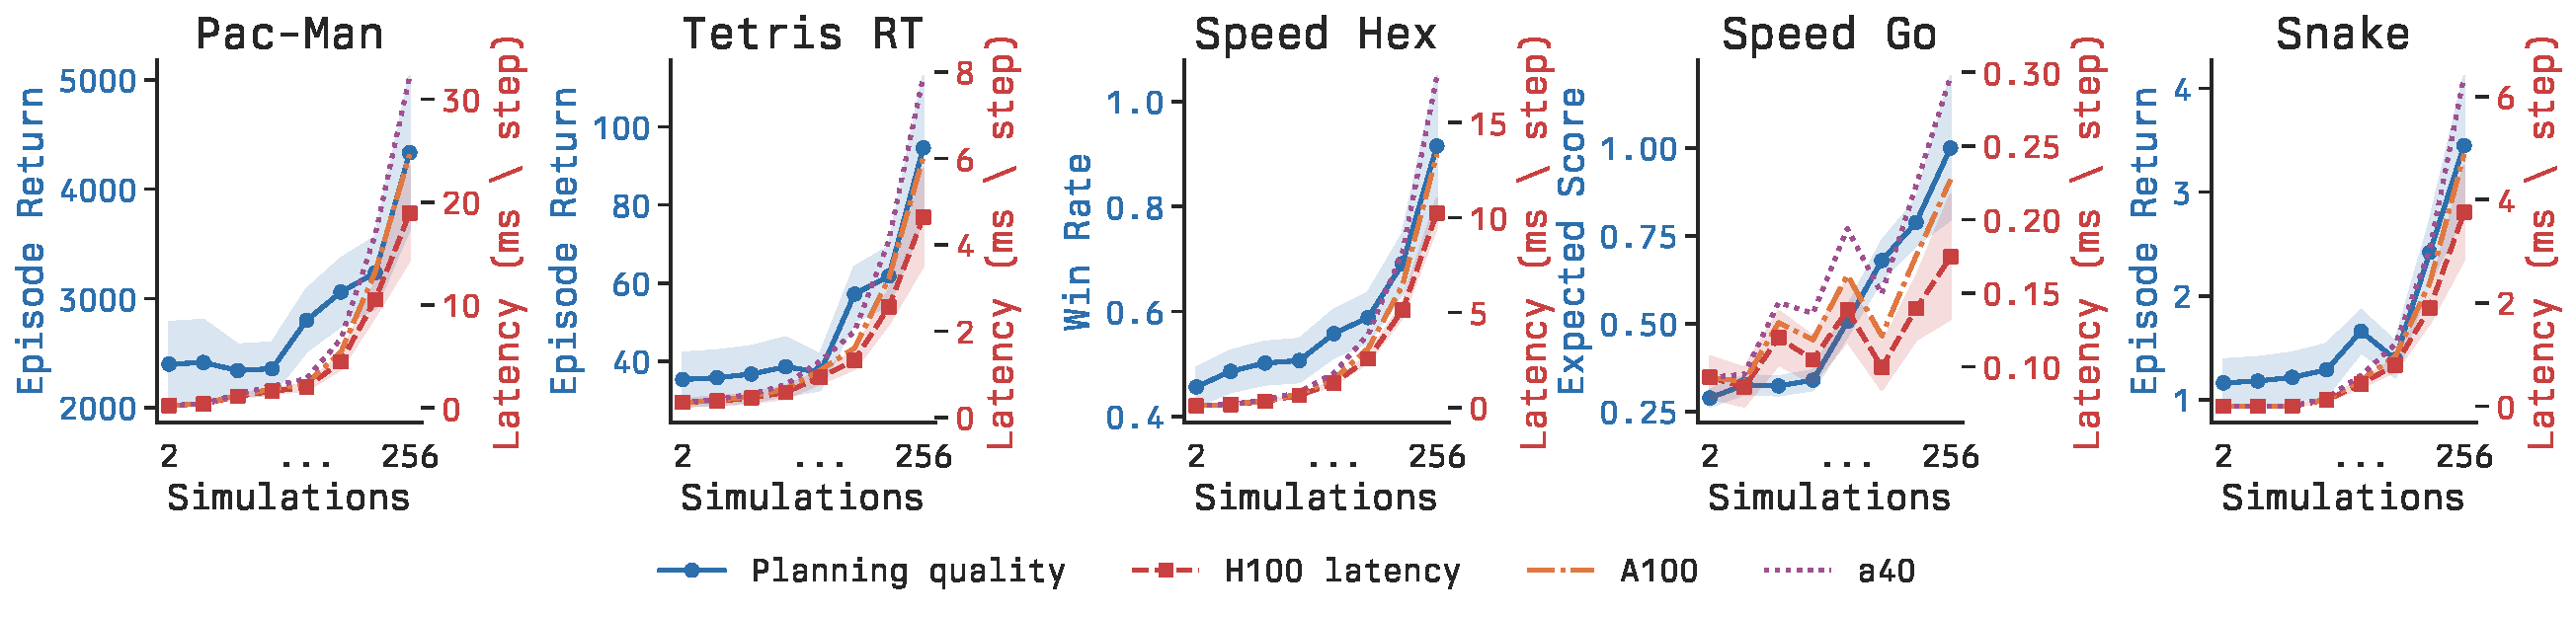
\includegraphics[width=\linewidth]{figures/scaling_appendix.pdf}
  \caption{Full co-scaling results across Pac-Man, real-time Tetris, Speed
    Hex, Speed Go, and Snake. Blue denotes planning quality; dashed curves
    denote per-step latency on H100, A100, and A40; shading shows $\pm$SE.}
  \label{fig:scaling_appendix}
\end{figure}

\begin{figure}[h]
  \centering
  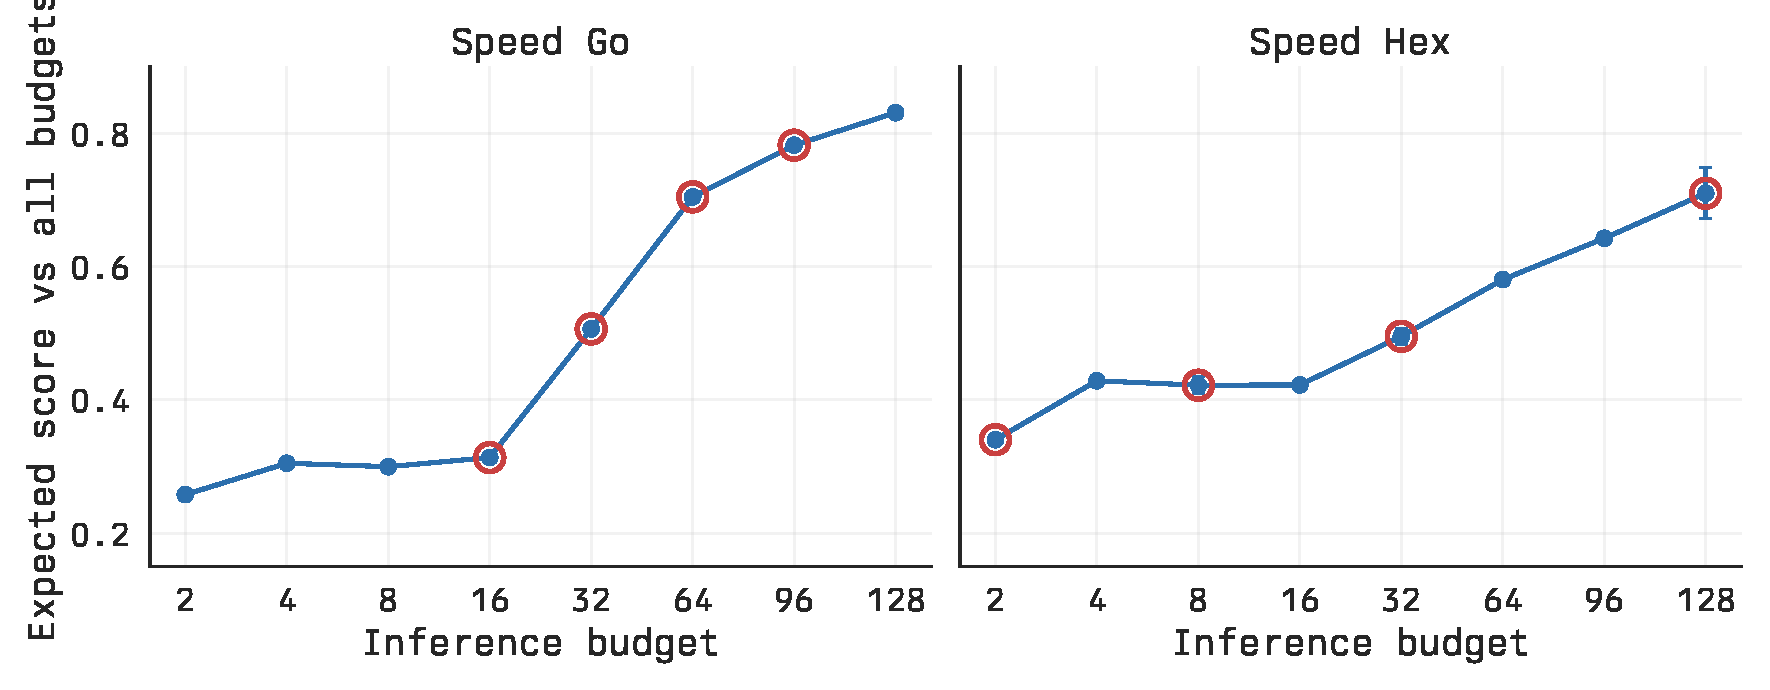
\includegraphics[width=\linewidth]{figures/clock_budget_calibration_go_hex.pdf}
  \caption{
    Simulation-option calibration for the two clock environments.
    Each point shows a budget's average expected score against all other
    candidate budgets.
    Red circles mark the options used in our clocked experiments:
    16/32/64/96 simulations for Speed Go and 2/8/32/128 for Speed Hex.}
  \label{fig:clock_budget_calibration}
\end{figure}


\section{Cross-Evaluation and Base Model Selection}
\label{app:cross_eval}

For the committed-action environments, we trained four AlphaZero checkpoints at
budgets $K \in \Kset$ and evaluated all 16 (train-$K$, eval-$K$) combinations.
Here, train-$K$ denotes the action-delay budget used during training, while
eval-$K$ denotes the action-delay budget used at test time.
For each train-$K$ checkpoint we additionally swept the MCTS simulation budget at
evaluation time and report the best raw episode return achieved for each eval-$K$.
The evaluation sweeps were: Tetris RT with simulation counts
$\{32, 64, 96, 128\}$, Pac-Man with $\{8, 16, 32, 64, 96, 128\}$, and Snake
with $\{32, 64, 96, 128\}$.

\begin{table}[h]
  \centering
  \small
  \setlength{\tabcolsep}{5pt}
  \begin{tabular}{llcccc}
    \toprule
    Environment & Train-$K$ & Eval-$K{=}1$ & Eval-$K{=}2$ & Eval-$K{=}3$ & Eval-$K{=}4$ \\
    \midrule
    \multirow{4}{*}{Tetris RT}
      & $K{=}1$ & 61.8 @ 128 & \textbf{85.0 @ 128} & \textbf{73.2 @ 128} & \textbf{69.0 @ 128} \\
      & $K{=}2$ & 30.0 @ 96  & 11.4 @ 128          & 7.4 @ 96            & 3.6 @ 96 \\
      & $K{=}3$ & \textbf{72.2 @ 128} & 22.0 @ 128 & 15.2 @ 128 & 11.8 @ 128 \\
      & $K{=}4$ & 69.6 @ 128 & 24.0 @ 96           & 23.2 @ 128          & 18.8 @ 128 \\
    \midrule
    \multirow{4}{*}{Pac-Man}
      & $K{=}1$ & \textbf{3235.4 @ 128} & 925.3 @ 128 & \textbf{2579.3 @ 128} & \textbf{1869.2 @ 96} \\
      & $K{=}2$ & 2458.5 @ 128 & 630.7 @ 128 & 866.7 @ 128 & 574.4 @ 96 \\
      & $K{=}3$ & 2749.7 @ 128 & 1122.3 @ 128 & 1110.6 @ 64 & 1051.2 @ 128 \\
      & $K{=}4$ & 2904.1 @ 128 & \textbf{1161.2 @ 128} & 1117.2 @ 128 & 1132.4 @ 96 \\
    \midrule
    \multirow{4}{*}{Snake}
      & $K{=}1$ & 0.77 @ 128 & 0.33 @ 128 & 0.50 @ 128 & 0.27 @ 128 \\
      & $K{=}2$ & 2.32 @ 128 & 0.56 @ 128 & 0.84 @ 128 & 0.31 @ 96 \\
      & $K{=}3$ & \textbf{2.42 @ 128} & \textbf{0.80 @ 64} & \textbf{1.13 @ 128} & \textbf{0.49 @ 96} \\
      & $K{=}4$ & 0.05 @ 32  & 0.05 @ 128 & 0.06 @ 128 & 0.07 @ 128 \\
    \bottomrule
  \end{tabular}
  \caption{
    Cross-evaluation of committed-action base models.
    Entries report the best raw episode return for each train-$K$/eval-$K$
    combination after optimizing over the evaluation simulation-budget sweep;
    the selected simulation count is shown after the `@' symbol. Bold marks the
    best train-$K$ for each eval-$K$ within an environment.}
\end{table}

The resulting pattern is environment-dependent but clear.
For Tetris RT, $K{=}1$ is the strongest base model overall: although the
$K{=}3$ checkpoint is best at eval-$K{=}1$, the $K{=}1$ checkpoint wins at
eval-$K \in \{2,3,4\}$ and has the highest mean return when averaging the
best-per-eval-$K$ scores.
For Pac-Man, $K{=}1$ also wins overall, dominating eval-$K \in \{1,3,4\}$ and
achieving the highest average performance across eval budgets, while $K{=}4$
is only slightly better at eval-$K{=}2$.
Snake differs qualitatively: the $K{=}3$ checkpoint is the strongest across all
four eval budgets and therefore serves as the frozen base model in that domain.

These results match the intuition that low-delay training is often causally
cleaner, since less delay-induced mismatch enters the value targets.
In addition, committed actions during delay steps are drawn from the base
model's policy, so a stronger base policy also produces better intermediate
states before the final MCTS action lands.
Accordingly, we use the $K{=}1$ checkpoint as the frozen base for Pac-Man and
Tetris RT, and the $K{=}3$ checkpoint for Snake.

\section{Strategy Profiles Across Environments}
\label{app:strategy_appendix}

\begin{figure}[t]
  \centering
  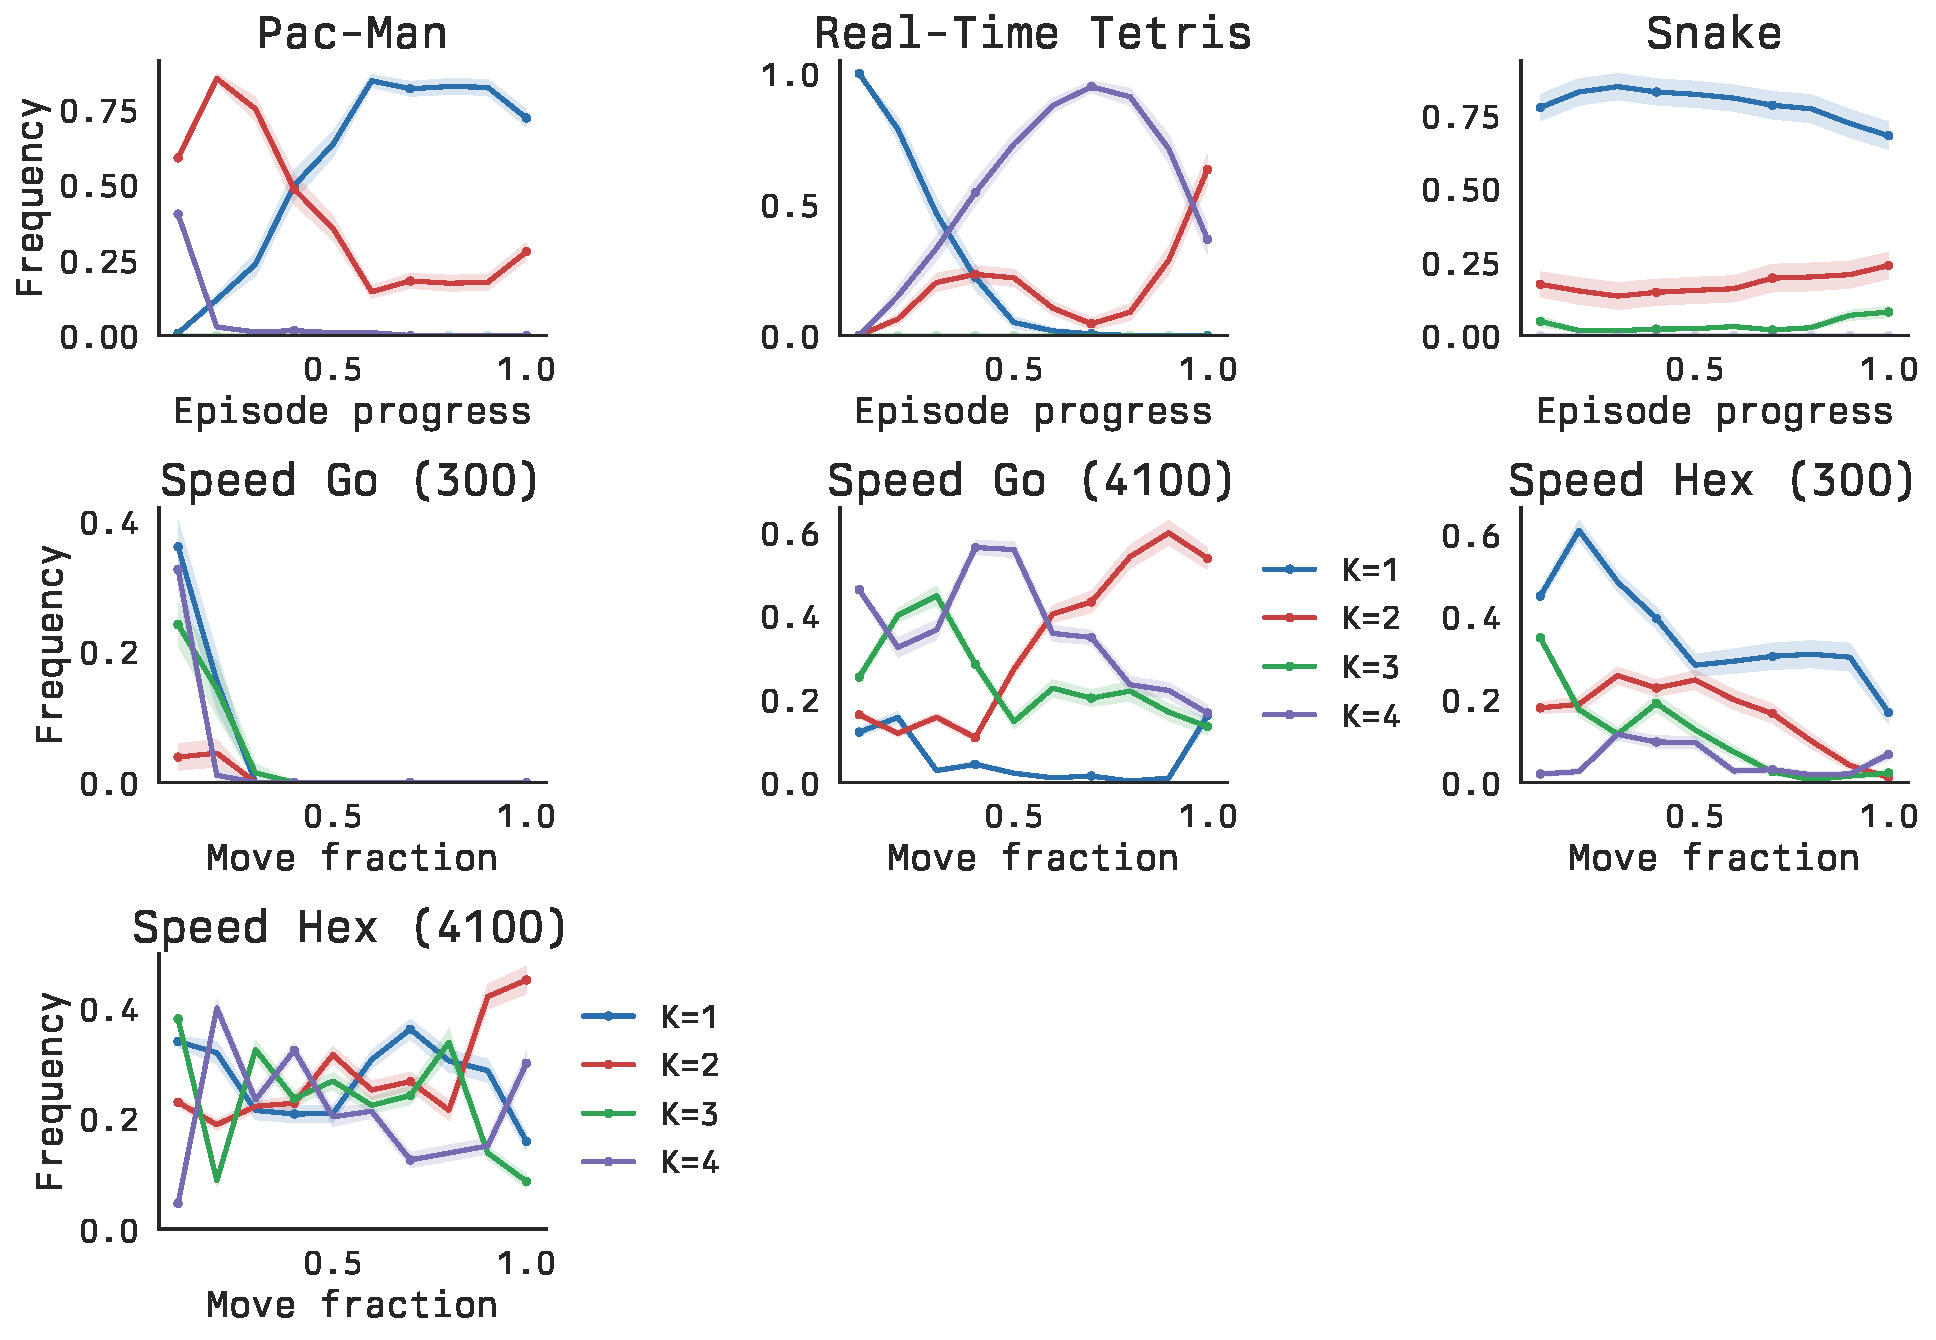
\includegraphics[width=\linewidth]{figures/strategy_appendix.pdf}
  \caption{Different environments induce different allocation profiles. Pac-Man
    becomes more reactive later in the episode, Tetris shifts toward deeper
    planning as the board densifies, Snake remains mostly reactive with occasional
    deeper planning in constrained states, and both clock games become less
    reactive when more time is available. This figure complements
    Figure~\ref{fig:strategy} by showing the full cross-environment strategy
    profiles rather than only the clock-game comparison.}
  \label{fig:strategy_appendix}
\end{figure}


\section{Strict-Timeout Speed Hex Control}
\label{app:hex_timeout_control}

The main Speed Hex setup allows the game to continue after the acting side exhausts
its remaining clock budget, so the experiment measures \emph{resource allocation}
rather than a pure timeout-avoidance game. To verify that this distinction matters,
we ran a strict-timeout control in which overspending the selected search budget
causes an immediate loss and there is no fallback behavior.

\begin{figure}[t]
  \centering
  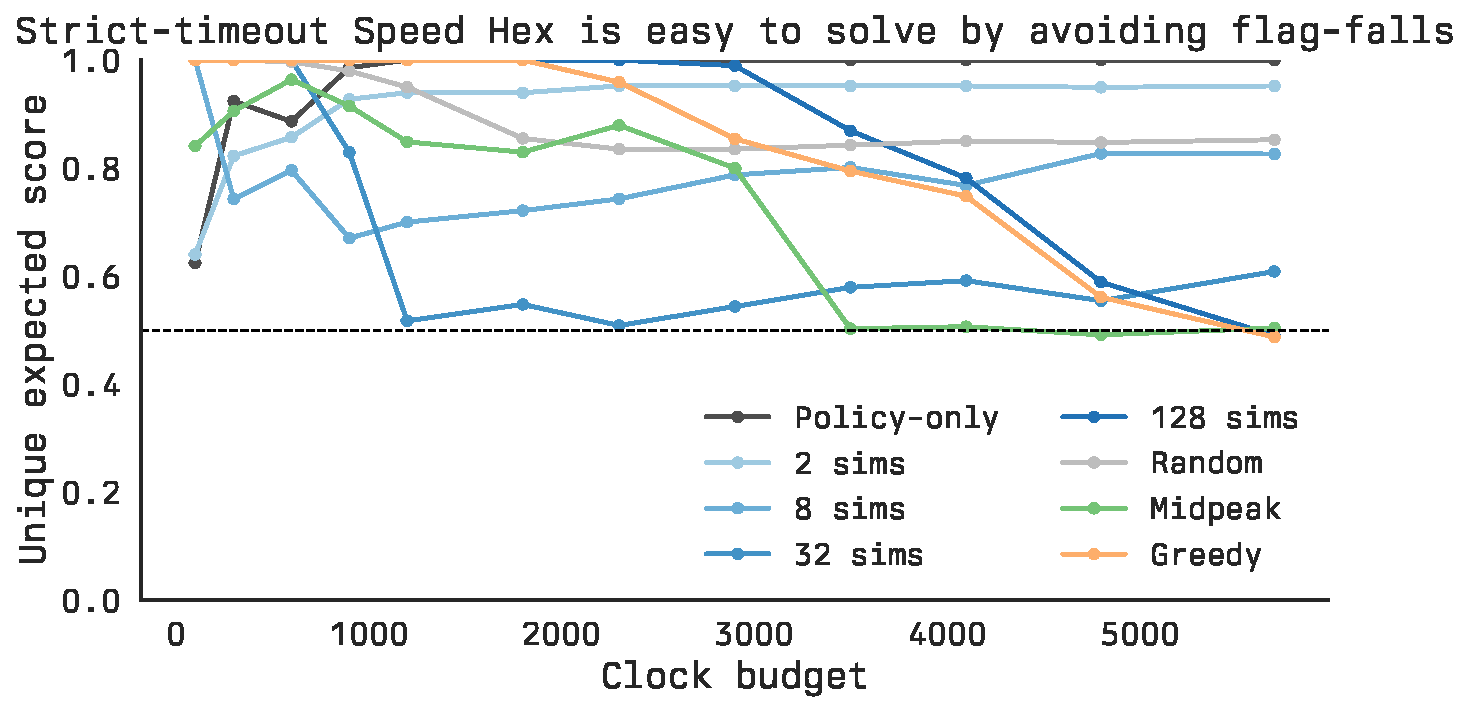
\includegraphics[width=\linewidth]{figures/hex_timeout_appendix.pdf}
  \caption{Strict-timeout Speed Hex is substantially easier than the main Speed Hex
    benchmark. Using the unique-game expected-score metric, the learned gate remains
    above parity against every opponent on average, with means of 0.952 against the
    policy-only opponent, 0.903 against fixed 2-simulation play, 0.904 against random
    allocation, and 0.893 even against the fixed 128-simulation opponent. At large
    budgets, the more aggressive opponents become the weakest because they overspend
    clock and lose on time.}
  \label{fig:hex_timeout_appendix}
\end{figure}

Figure~\ref{fig:hex_timeout_appendix} shows the resulting per-budget head-to-head
curves under the unique-game metric used in the main paper. The learned gate stays
above parity against every opponent \emph{on average}, and against five of the eight
opponents it is above parity at \emph{every} evaluated budget. Even the hardest
fixed-budget baseline under this metric, always-32, averages only 0.690 against the
gate, while policy-only averages 0.952 and random allocation averages 0.904. The
only sub-parity points occur for the more clock-aggressive baselines at the largest
budgets: fixed 128-simulation play dips to 0.490 at $T{=}5700$, midpeak dips to
0.491 at $T{=}4800$, and greedy dips to 0.487 at $T{=}5700$. This pattern is the
opposite of what we observe in the main benchmark. Once timeout is an immediate
terminal event, stronger search is no longer reliably beneficial; it often just
increases the probability of burning too much clock. In other words, the game becomes
easier because the gating policy can win largely by learning a conservative
time-management rule rather than by solving the underlying Hex positions more
effectively.


\section{Implementation Details}
\label{app:implementation}

\subsection{Gating network architecture}

\textbf{Spatial branch.}
The game grid is processed by a $1{\times}1$ convolution lifting to 64 channels,
followed by three residual blocks with Layer Normalization and global average pooling
to a 64-dimensional spatial representation.
Layer Normalization is used because the gating policy operates on a single environment
instance per rollout step, making batch statistics undefined.

\textbf{Time / clock embedding.}
For committed-action environments, the normalized step count is encoded as a 2-vector
and projected through a small MLP before being added to the spatial features.
For clock environments, the remaining clock fraction is similarly embedded and added.

\textbf{Fusion and heads.}
The spatial representation (64-dim), planner trunk features (128-dim), and planner
value (1-dim) are concatenated and passed through dual MLP heads: a policy head
producing logits over $K$, and a value head producing a scalar baseline.

\textbf{Speed Hex gating network.}
Uses a GRU backbone rather than a feedforward network, maintaining a recurrent hidden
state across moves within each game to track temporal context.

\subsection{Training hyperparameters}

\begin{table}[h]
  \centering
  \caption{PPO hyperparameters for committed-action environments.}
  \label{tab:hparams}
  \begin{tabular}{lcc}
    \toprule
    Hyperparameter & Pac-Man & Tetris RT \\
    \midrule
    Num.\ parallel envs     & 32   & 32   \\
    Meta-steps per rollout  & 384  & 384  \\
    PPO epochs per rollout  & 4    & 4    \\
    Num.\ mini-batches      & 16   & 16   \\
    Meta-reward mode        & raw  & raw  \\
    Discount $\gamma$       & 0.99 & 0.99 \\
    GAE $\lambda$           & 0.95 & 0.95 \\
    PPO clip $\epsilon$     & 0.2  & 0.2  \\
    Entropy coefficient     & 0.01 & 0.01 \\
    Learning rate           & 3e-4 & 3e-4 \\
    Sim options             & 32, 64, 96, 128 & 32, 64, 96, 128 \\
    \bottomrule
  \end{tabular}
\end{table}

\subsection{JAX implementation and batching strategy}

The main computational challenge is that our system nests a meta-policy on top of
an AlphaZero-style planner, so a naive implementation would repeatedly invoke MCTS
inside an outer RL loop with substantial Python overhead. Our implementation avoids
this by pushing nearly all control flow into JAX primitives.

\textbf{Base planner training.}
The frozen planners are trained with our own Gumbel-AlphaZero stack built on top of
the Jumanji environments, using
\texttt{mctx.gumbel\_muzero\_policy} for search. Within each planner step, the MCTS
simulations are executed inside a compiled \texttt{lax.scan}; leaf expansion and
backup are batched across parallel environments with \texttt{vmap}; and the full
self-play/training pipeline is wrapped in \texttt{jit}. In the multi-device setting,
the leading batch dimension is sharded with \texttt{pmap}, so each accelerator runs
the same compiled self-play/update program on its local slice of environments.

\textbf{Gating-policy training.}
For the gating layer, we again compile whole rollouts rather than individual steps.
Each PPO rollout is one \texttt{jit}-compiled \texttt{lax.scan} over meta-decisions,
and advantage computation is another reverse \texttt{lax.scan}. The recurrent Speed
Hex gate uses the same pattern: the GRU unroll is expressed as a scan, while PPO
operates on sequence chunks rather than on Python loops over timesteps.

\textbf{Evaluating all budget options in parallel.}
The key batching trick is that, during gating training and evaluation, we compute
the transition for every available budget option at each meta-step and only then
select the branch corresponding to the gate's chosen action. Concretely, for
$K \in \{1,2,3,4\}$ we run all four \texttt{meta\_step\_one\_k} branches, stack the
resulting rewards, discounts, next states, and next observations, and use a batched
selection operator to pick the chosen branch per environment. This spends extra
compute relative to evaluating only the selected option, but it preserves static
shapes, keeps the whole computation batched, and avoids recompilation or Python-side
control flow. In practice this systems tradeoff is what makes the meta-MCTS stack
fast enough to train routinely rather than as a one-off systems effort.

\textbf{Practical effect.}
These engineering choices --- \texttt{mctx} for search, \texttt{vmap} for environment
parallelism, \texttt{jit} for whole-program compilation, \texttt{pmap} for device
parallelism, and \texttt{lax.scan} for both MCTS inner loops and PPO rollout loops ---
reduce wall-clock training time dramatically. In our internal runs, the end-to-end
training workflow dropped from roughly two weeks in an earlier less-batched pipeline
to roughly six hours in the optimized JAX implementation. The full implementation is
included in our anonymous code submission.


\section{Detailed Two-GPU Deployment Breakdown}
\label{app:deployment_details}

We ran the full asynchronous deployment grid for all 45 settings:
3 environments (Tetris, Pac-Man, Snake) $\times$ 3 GPUs (H100, A100, A40)
$\times$ 5 frame rates (8--12\,FPS).
Figure~\ref{fig:deployment_appendix} gives the complete breakdown by environment,
GPU, and FPS for return, deadline miss rate, and p95 slack to deadline.

Several patterns are clear.
First, H100 is consistently reliable across the entire tested range.
In Tetris its miss rate stays at $0.014\%$ for all FPS values, with p95 slack
remaining positive from $+291.0$\,ms at 8\,FPS to $+123.6$\,ms at 12\,FPS.
Snake is even easier: H100 and A100 stay at $0.001\%$ miss rate throughout, and
A40 stays at or below $0.005\%$.

Second, the deployment boundary appears where slack collapses.
Tetris on A40 is the clearest example: p95 slack decreases monotonically from
$+162.2$\,ms (8\,FPS) to $-4.1$\,ms (12\,FPS), and the miss rate jumps from
$0.046\%$ to $50.669\%$.
By contrast, Tetris on A100 remains usable even at 12\,FPS, with p95 slack still
positive at $+24.5$\,ms and miss rate only $0.188\%$.

Third, Pac-Man is the most timing-sensitive environment.
Even with positive p95 slack throughout, A100 and A40 exhibit non-trivial miss
rates across all FPS values.
At 12\,FPS, Pac-Man reaches $30.369\%$ misses on A100 and $13.073\%$ on A40,
whereas H100 stays much lower at $3.927\%$.
This indicates that for Pac-Man, the far latency tail beyond the p95 threshold
matters operationally even when the central mass remains in-budget.

Finally, return remains comparatively stable over a broad deployment range despite
these timing differences.
Tetris returns remain in the $41$--$50$ range on H100/A100 and in the high-30s to
low-40s on A40 except at the most constrained settings.
Pac-Man degrades more gradually with hardware and FPS than its miss-rate curve might
suggest, while Snake is nearly flat across all tested settings.
Together these results support the main-text conclusion: the committed-action
training protocol transfers robustly to asynchronous hardware deployment, and the
observed failures emerge in predictable deadline-limited regimes rather than as
qualitatively new behaviors.

\begin{figure}[h]
  \centering
  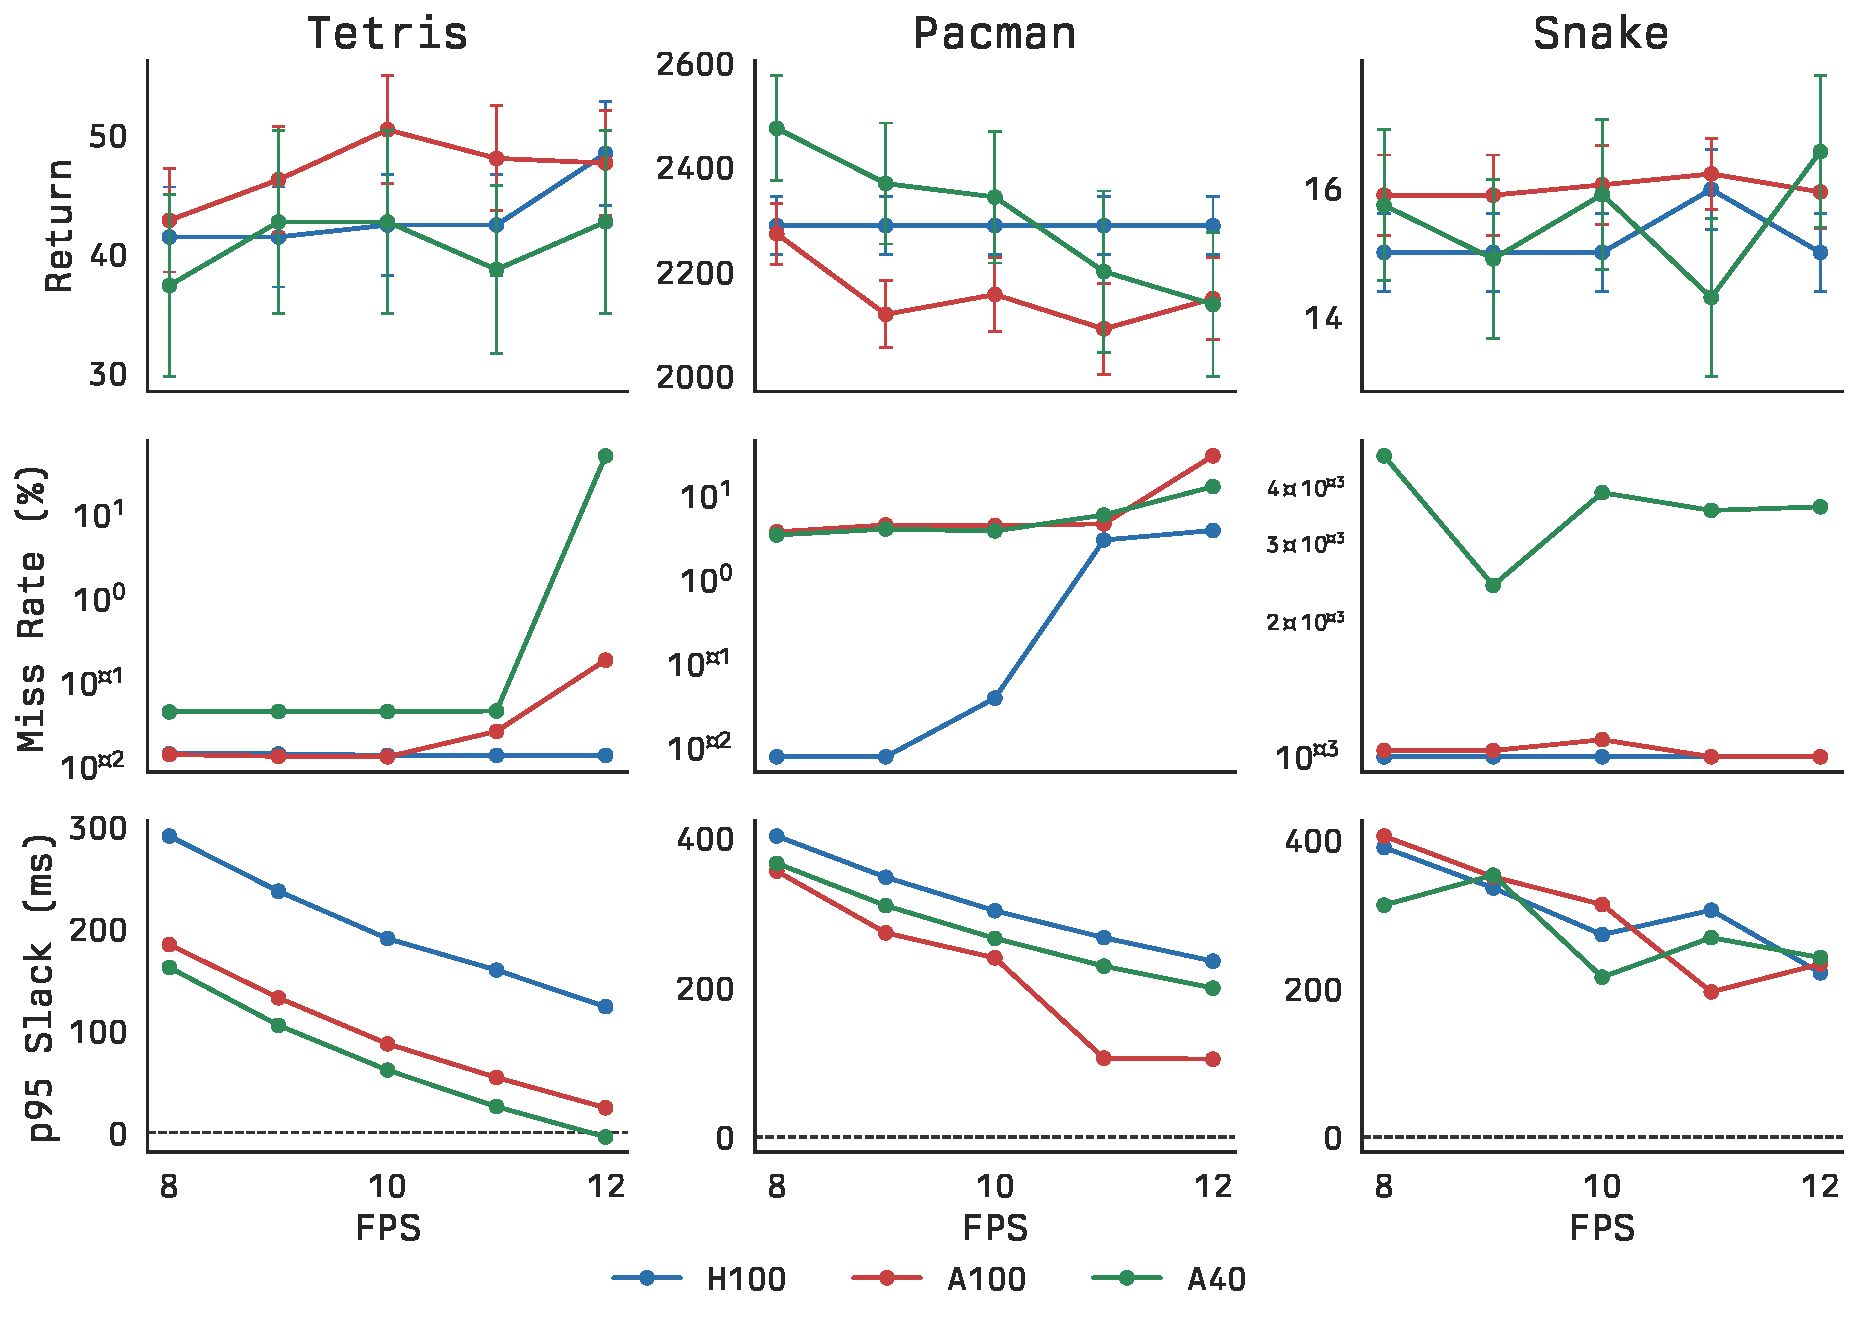
\includegraphics[width=\linewidth]{figures/deployment_appendix.pdf}
  \caption{Detailed two-GPU deployment breakdown across Tetris, Pac-Man, and Snake.
    Top: return vs.\ FPS. Middle: deadline miss rate. Bottom: p95 slack to the
    $K{=}4$ deadline. Snake remains robust, Tetris fails only near the tightest
    A40 regime, and Pac-Man is the most latency-sensitive.}
  \label{fig:deployment_appendix}
\end{figure}


\section{Additional Results and Ablations}
\label{app:ablations}

We also ran input-ablation evaluations for the committed-action environments, in
which the gating policy received zeroed observation features, zeroed time
features, zeroed planner trunk features, or a zeroed planner value input while
the environment dynamics and MCTS planner remained unchanged.
Across environments, ablating planner trunk features was consistently
disruptive, while zeroing the scalar value input had only minor effect; in
Tetris, zeroing either the board observation or planner trunk substantially
reduced return, while in Pac-Man and Snake the learned behavior was more robust
to removing any single input channel.

\begin{table}[h]
  \centering
  \small
  \setlength{\tabcolsep}{6pt}
  \begin{tabular}{lccccc}
    \toprule
    Environment & Baseline & Zero obs & Zero time & Zero trunk & Zero value \\
    \midrule
    Pac-Man   & 2245.6 & 2379.2 & 1571.2 & 1812.6 & 2189.8 \\
    Tetris RT &   44.0 &   34.4 &   37.6 &   33.2 &   44.0 \\
    Snake     &   15.18 &  14.92 &  15.94 &  15.66 &  16.14 \\
    \bottomrule
  \end{tabular}
  \caption{
    Input-ablation results for the committed-action gating policies.
    Entries report mean episode return under each ablation condition while the
    environment and MCTS planner remain unchanged.}
\end{table}

%%%%%%%%%%%%%%%%%%%%%%%%%%%%%%%%%%%%%%%%%%%%%%%%%%%%%%%%%%%%

\section{Real-Time RL, SMDPs, and Committed-Action Training}
\label{app:rtrl_smdp}

\subsection*{The RTRL framework and its single-step restriction}

\citet{ramstedt2019rtrl} formalise real-time interaction via the
\emph{Real-Time Markov Decision Process} (RTMDP), which augments the environment
state with the action currently in execution:
$\mathbf{x}_t = (s_t, a_t)$,
where $a_t$ was selected one step earlier based on $s_{t-1}$.
The transition is
$p(\mathbf{x}_{t+1} \mid \mathbf{x}_t, \hat{a}_t) =
 p(s_{t+1} \mid s_t, a_t)\,\delta(a_{t+1} - \hat{a}_t)$,
passing the newly selected action $\hat{a}_t$ forward as the next state component.
This is equivalent to a \emph{constant 1-step delay MDP}~\citep{walsh2009delayed}:
the action the agent emits is applied one timestep later, and the policy must
learn to predict where the state will be when the action lands.

The framework is well-suited for lightweight policies whose evaluation time
fits within one frame.
For MCTS planning, however, the computation budget spans $K \in \{1,2,3,4\}$
frames ($111$--$444$\,ms at 9\,FPS).
A direct extension to a $K$-step delay MDP would require augmenting the state
with the $K$ most recent actions,
$\mathbf{x}_t = (s_t, a_{t-K+1}, \ldots, a_t)$,
whose size grows with planning budget.
Worse, under \emph{variable} $K$ the augmented state space would change
dimensionality at each meta-step, and the policy would need to predict the
state $K$ steps ahead through a chain of arbitrary committed actions---a
hard credit-assignment problem that does not arise in the 1-step case.

\subsection*{Training is a discrete SMDP; deployment is a genuine SMDP}

\paragraph{Simulation.}
In training the environment is synchronous: MCTS runs in zero simulated time.
Each meta-step proceeds by (1) gating chooses $K$, (2) $K{-}1$ committed
argmax steps execute, (3) the MCTS result is applied.
From the meta-policy's perspective this is a
\emph{Semi-Markov Decision Process}~\citep{puterman1994mdp} with \emph{deterministic}
holding time $\tau = K$ (chosen by the meta-action).
Successive meta-decisions are spaced $K$ environment steps apart and the
appropriate discount is $\gamma^K$, which is exactly the discount applied
in training.
Formally this is a discrete SMDP with options~\citep{sutton1999between}:
each $(K, \pi_{\mathrm{reflex}})$ pair defines an option of length $K$ terminating
with the MCTS action.

\paragraph{Deployment.}
In real-time deployment the holding time between meta-decisions equals
$K \times T_{\mathrm{frame}}$: MCTS runs concurrently on GPU~1 while the
environment executes the $K$ reflex frames on GPU~0, so the two durations
\emph{overlap} rather than sum.
Given $K$, the elapsed wall-clock time is $K \times T_{\mathrm{frame}}$
regardless of MCTS latency, provided search completes within the deadline.
The holding time is stochastic only because $K$ is chosen stochastically
by $\pigate$; this is a true SMDP in the continuous-time
sense~\citep{puterman1994mdp}.
Our measurements confirm that MCTS latency stays well within the frame budget\footnote{Note the distinction between \emph{frame budget} and \emph{planning budget} $K$. The frame budget is the time between frames}
(H100: mean $122$\,ms, p95 $205$\,ms; A40: mean $197$\,ms, p95 $338$\,ms
vs.\ a $K{=}4$ frame budget of $444$\,ms at 9\,FPS), so the deterministic
simulation discount $\gamma^K$ matches the deployment discount closely,
which is why sim-to-real transfer succeeds without retraining.

\subsection*{How committed-action training avoids state augmentation}

The central reason the $K$-step RTMDP state augmentation is unnecessary in
our framework is that \emph{the committed action at each intermediate step is
computed from the current state, not from a state $K$ steps ago}.
Specifically, the committed action at frame $t$ is
$a_t = \arg\max_a \pi_\theta(a \mid s_t)$, evaluated fresh in $\sim$2\,ms---well
within the $111$\,ms frame budget.
Only the MCTS result is stale: it was computed on $s_0$ (start of meta-step)
but applied at $s_K$ (after $K{-}1$ committed steps).
This staleness is explicitly modeled in training: the $K{-}1$ committed steps
actually execute in the environment before the MCTS action lands, so the policy
learns to handle the $K$-step gap without any state augmentation.

In the RTRL vocabulary, the committed-action component operates in the
\emph{turn-based} regime (computation time $\ll$ frame time, so the environment
effectively pauses during action selection), while the MCTS component operates
in a $K$-step delay regime whose effects are absorbed by the training curriculum
rather than by augmenting the state space.
The key property that makes this possible---and that the standard RTMDP does not
exploit---is that the intermediate policy $\pi_{\mathrm{reflex}}$ is a
\emph{deterministic function of the current state}, so its actions do not need
to be carried in the state to recover the Markov property.

%%%%%%%%%%%%%%%%%%%%%%%%%%%%%%%%%%%%%%%%%%%%%%%%%%%%%%%%%%%%

\newpage
\input{checklist.tex}

\end{document}

